% PLEASE USE THIS FILE AS A TEMPLATE
% Check file iosart2x.tex for more examples

% add. options: [seceqn,secthm,crcready,onecolumn]
\documentclass[sw]{iosart2x}
	\usepackage{hyperref}
	\usepackage{listings}
	
	\usepackage{multirow}
	
	\usepackage{color}
	\newcommand{\pc}[1]{\noindent\textcolor{red}{\{Pieter says: #1{\bf \}}}}
	%\usepackage{dcolumn}
	%\usepackage{endnotes}
	
	%%%%%%%%%%% Put your definitions here
	
	
	%%%%%%%%%%% End of definitions
	
	\pubyear{0000}
	\volume{0}
	\firstpage{1}
	\lastpage{1}
	
	\begin{document}
	\sloppy
	\begin{frontmatter}
	
	%\pretitle{}
	\title{Publishing and archiving planned and live public transport events with the Linked~Connections framework}
	\runningtitle{Publishing and archiving planned and live public transport events with the Linked~Connections framework}
	%\subtitle{}
	
	% For one author:
	%\author{\inits{N.}\fnms{Name1} \snm{Surname1}\ead[label=e1]{first@somewhere.com}}
	%\address{Department first, \orgname{University or Company name},
	%Abbreviate US states, \cny{Country}\printead[presep={\\}]{e1}}
	%\runningauthor{N. Surname1}
	
	% Two or more authors:
	\author[A]{\inits{J.}\fnms{Julian} \snm{Rojas}\ead[label=e1]{julianandres.rojasmelendez@ugent.be}},
	\author[B]{\inits{D.}\fnms{David} \snm{Chaves-Fraga}\ead[label=e2]{dchaves@fi.upm.es}},
	\author[A]{\inits{P.}\fnms{Pieter} \snm{Colpaert}\ead[label=e3]{pieter.colpaert@ugent.be}},
	\author[B]{\inits{O.}\fnms{Oscar} \snm{Corcho}\ead[label=e4]{ocorcho@fi.upm.es}}
	and
	\author[A]{\inits{P.}\fnms{Ruben} \snm{Verborgh}\ead[label=e5]{ruben.verborgh@ugent.be}}
	\runningauthor{J. Rojas et al.}
	\address[A]{IDLab, Department of Electronics and Information Systems, \orgname{Ghent University-imec}, \cny{Belgium}}
	\address[B]{Ontology Engineering Group, \orgname{Universidad Polit\'ecnica de Madrid}, \cny{Spain}
	  \printead[presep={\\}]{e1,e2,e3,e4,e5}}
	
	%\begin{review}{editor}
	%\reviewer{\fnms{First} \snm{Editor}\address{\orgname{University or Company name}, \cny{Country}}}
	%\reviewer{\fnms{Second} \snm{Editor}\address{\orgname{First University or Company name}, \cny{Country}
	%    and \orgname{Second University or Company name}, \cny{Country}}}
	%\end{review}
	%\begin{review}{solicited}
	%\reviewer{\fnms{First} \snm{Solicited reviewer}\address{\orgname{University or Company name}, \cny{Country}}}
	%\reviewer{\snm{anonymous reviewer}}
	%\end{review}
	%\begin{review}{open}
	%\reviewer{\fnms{First} \snm{Open Reviewer}\address{\orgname{University or Company name}, \cny{Country}}}
	%\end{review}
	
	\begin{abstract}
	  % Context
	  Using Linked Data based approaches, companies and institutions are seeking ways to automate the adoption of Open Datasets.
	  In the transport domain, data about planned events, live updates and historical data have to coexist to provide reliable data to route planning assistants.
	  % Need
	  Linked Connections (LC) introduces a preliminary specification that allows cost-efficient publishing of the raw public transport data in linked information resources.
	  % Task
	  This paper gives an overview of Linked Connections so far and supports claims with existing and novel experiments.
	  %Object
	  Furthermore,
	  (i) an extension of the current Linked Connections specification providing methods and vocabulary to deal with live data is provided;
	  (ii) a Linked Connections Live server is developed that is able to process GTFS-RT feeds providing consistent identifiers; and
	  (iii) an efficient management of historical data taking into account the size of each fragments exposed on the Web is described.
	  % Findings
	  We discover that the size of the fragments has a relevant impact on the performance of query evaluation.
	  Based on our experiments conducted in 2018, an ideal Linked Connections fragment -- for the use case of route planning with the current client -- weighs about 50kb.
	  % Conclusion and perspective
	  This research scratches the surface on a Web ecosystem for route planning.
	  In future works, we envision to find optimal fragmentation strategies of larger public transit networks for automated federated route planning.
	\end{abstract}
	
	\begin{keyword}
	\kwd{Linked Connections}
	\kwd{Historical Data}
	\kwd{Real time data}
	\kwd{Reliable data}	
	\kwd{Linked Data Fragments}
	\end{keyword}
	
	\end{frontmatter}
	
	%%%%%%%%%%% The article body starts:
	
	%\section{}\label{s1}
	
	%\subsection{}\label{s1.1}
	\section{Introduction}\label{introduction} %Oscar and David
	In the current state of the Web of Data, a wide amount of that data are exposed following the principles of Linked Data~\cite{bizer2009linked}. Giving unique identifiers to each resource, representing the data using a shared and common vocabulary of a domain or the possibility of dereferencing each URI are some of the relevant aspects that made Linked Data as one the most common approaches to organize and expose the data on the Web~\cite{heath2011linked}. This features allow third parties to query the data in a standard way, using for example, the corresponding query language for RDF, SPARQL~\cite{prud2006sparql}, and the possibility of doing federation across multiple datasets~\cite{buil2013federating}. However, today, a lot of domains need to deal with live and historical data where is important to maintain stable identifiers that remain valid over time. The problems regarding the manage of these types of data and the relation with Linked Data have not widely researched. One of the most relevant domains where contributions will have a relevant impact is the transport domain, where a complex environment with multiple types of data sources have to be managed to provide reliable data to information systems.
	
	Since March 2017, one of the main motivations for developing solutions about multimodal and integrated travel information services is the publication of the new directive by the EU Commission about discoverability and access to public transport data across Europe\footnote{\url{https://ec.europa.eu/transport/sites/transport/files/2017-sustainable-urban-mobility-policy-context.pdf}}. This document proposes the making of public transport data from providers available on national or common access points saved on databases, data warehouse or repositories. All the states will provide access to a unique common point following different static standards as Transmodel\footnote{\url{http://www.transmodel-cen.eu}}, Datex II\footnote{\url{http://www.datex2.eu}} or GTFS\footnote{\url{https://developers.google.com/transit/gtfs}} and real-time standards like GTFS-RT\footnote{\url{https://developers.google.com/transit/gtfs-realtime/}} or SIRI\footnote{\url{http://www.transmodel-cen.eu/standards/siri/}}. So the domain requires solutions able to provide reliable data and to deal with the heterogeneity of access points and the data formats.
	
	One of the main challenges when the Linked Data approaches deal with transport domain, where live and historical data has to be taken into account for providing consistent data to the information services, is how to ensure that the identifiers of each resource is stable and valid over time. For example, if we define the connection entity as a departure-arrival pair, as has been done in previous works on Linked Connections~\cite{colpaert2015intermodal}, the URI of each connection was defined getting information from static GTFS datasets. At the moment that live data is involved, those URIs are not consistent because the live information creates new instances of a connection at different points in time. An example of the conceptualization of a connection is shown in the Figure \ref{fig:connection}. Other relevant challenge is how to manage the exposed historical data on the Web to allow an optimal query performance. One of the requirements of most relevant route planning algorithms is that the data have to be sorted by the time. In previous works of Linked Connections~\cite{rojas2017providing}, we developed a server that paginates the list of connections in departure time intervals (10 minutes) and publishes these pages over HTTP. We have noticed that the clients were able to analyze the historical data but the performance was too low.
	
	\begin{figure}[t]
		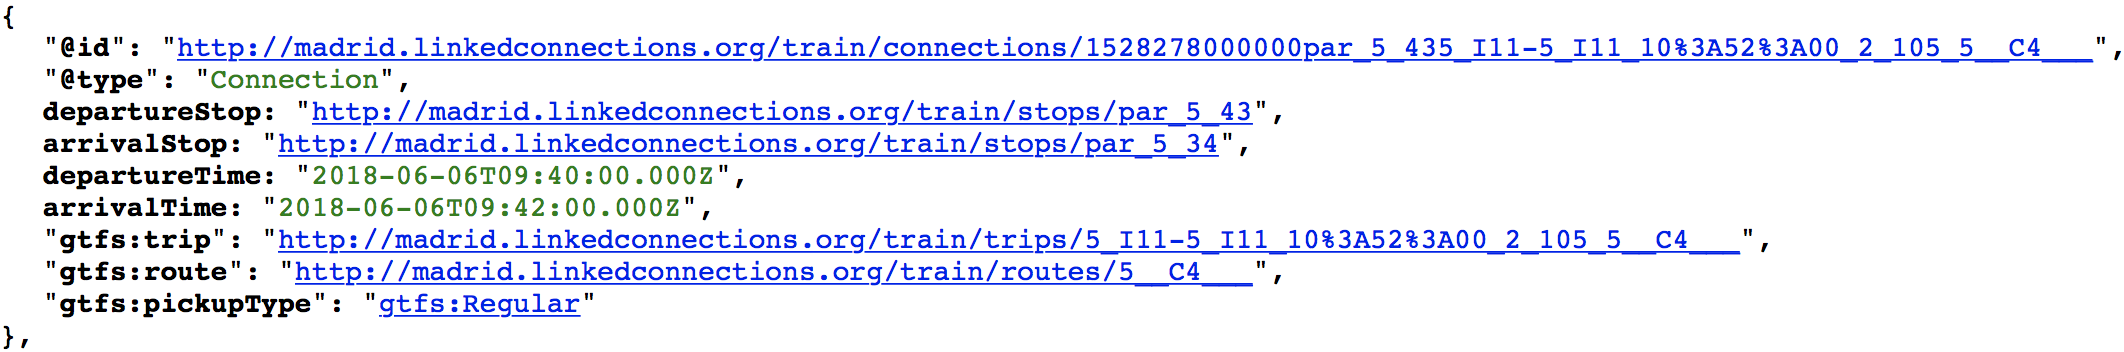
\includegraphics[height=0.08\textheight, width=0.47\textwidth]{images/connection.png}
		\caption{Example of a connection at LC in JSON-LD}\label{fig:connection}
	\end{figure}
	
	Our work is focused on providing an improvement of the current state of Linked Connections framework by allowing an efficient management of historical and live data with a standard vocabulary for the transport domain. This is relevant because of two main reasons: (i) currently, a lot of transport companies are starting to provide access to their live services, but the most common way to do it, is to develop an ad-hoc solution like APIs or web services that only work locally~\cite{colpaert2016public} and (ii) the heterogeneity of the domain in terms of data formats will be a very relevant problem next years, especially in Europe, based on the proposal of the EU Commission so a standard framework will be needed.  
	
	In this paper we present the Linked Connections framework to provide reliable access to live and historical data. Our main contribution is the extension of previous version of the LC server, by providing an efficient management of live and historical data. First, we develop a library that gets information from static GTFS datasets and GTFS-RT data streams and integrate them following the LC vocabulary. Second, we modify the approach of Linked Connections for splitting the fragments of the data using a specific size of each fragment instead of the time. Third, we program a route planning algorithm in the top of the LC server to test if our approach is able to provide reliable data. Finally, we evaluate the improvements comparing the new version of the LC framework with our previous approaches, as base line, and we analyse the impact of the fragment size in the performance of a route plan.
	
	The paper is organized as follows: Section 2 presents some of the related work about relevant approaches for exposing data on the web efficiently,  previous steps about the Linked Connections framework, a description of the \textit{de-facto} standard GTFS and the specification of relevant route planning algorithms. Section 3 describes our proposal about the improvements of the Linked Connections framework and a working example description. Section 4 presents the design of our experiments. Section 5 describes the results we obtained evaluating our main contributions. Section 6 provides a brief discussion about the relevance of our contributions, and Section 7 presents conclusions and areas for future work.
	
	
	\section{Related Work}\label{related_work} %David
	On the current state of the Web, huge amount of data are exposed following the principles of Linked Data. In this section, we describe the main contributions on this topic focused on an efficient publication of data on the transport domain, a description of previous approaches developed using the Linked Connections framework and the analysis of the model for transport data that supports our work. Finally we analyse the most relevant algorithms for route planning.
	
	One of the most well-known alternatives to publish data on the Web is Linked Data~\cite{bizer2009linked}. Linked Data allows to identify in an unique way resources on the Web using identifiers, or HTTP URIs. It is a method to distribute and scale data over large organizations such as the Web. When looking up this identifier by using the HTTP protocol or using a Web browser, a definition must be returned, including links towards other related resources, a practice called \textit{dereferencing}. The triple format to be used in combination with URIs is standardized within RDF. The URIs used for these triples already existed in other data sources, and we thus favoured using the same identifiers. It is up to a data publisher to make a choice on which data sources can provide the identifiers for a certain type of entities. 
	
	A common problem in Linked Data is the availability of the triple stores. They provide a way to getting data using the SPARQL query language but at the moment of queries involving long periods of time, these approaches are not efficient~\cite{verborgh2014querying}. The Linked Data Fragments(LDF)~\cite{verborgh2016triple,verborgh2014web} solve this issue fragmenting the data in several HTTP documents. Following this approach the store moves the load from server side to client side improving its availability. Comunica~\cite{taelman2018comunica} is a framework that extends the possibilities of LDF, allowing to query other semantic interfaces as common SPARQL endpoint, RDF data dumps or HDT datasets~\cite{fernandez2013binary}. 
	
	Linked Connections~\cite{colpaert2015intermodal} applies this approach to develop a cost-efficient solution based on a HTTP interface for transport data. The main assumption of LC is that the relevant data for route planners can be based on the connection concept. Basically, as the LC vocabulary\footnote{\url{http://semweb.mmlab.be/ns/linkedconnections}} defines it, a connection describes a departure at a certain stop and an arrival at a different stop with their corresponding departure and arrival times and without any intermediate stop. A basic implementation of LC is shown in Figure \ref{fig:lc_imp}, where the route planning algorithms have to analyse the connections (small rectangles) through the pages (big rectangles) and across time to find the expected route. The join between the connections is possible because same resources have same identifiers, based on one of the principles of Linked Data. The Hydra Ontology~\cite{lanthaler2013hydra} is used to specify the next and previous page links as well as how the resource itself should be discovered
	
	
	\begin{figure}[t]
		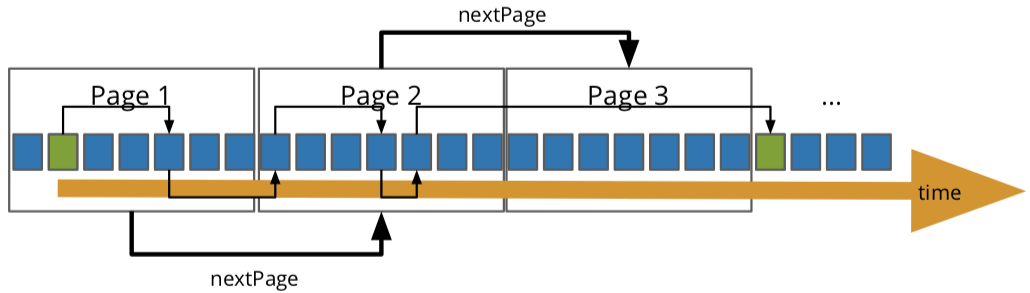
\includegraphics[width=0.47\textwidth]{images/implementation.png}
		\caption{Linked Connections implementation}\label{fig:lc_imp}
	\end{figure}
	
	It also relevant to describe the previous works that has been carried out using the specification of Linked Connections. For example, \cite{colpaert2017public} describes and analyses the behaviour of a basic transport API and the Linked Connections framework for public transit route planning, comparing the CPU and query execution time. The authors found that, at the expense of a higher bandwidth consumption, more queries can be answered using LC than the origin-destination API. In \cite{colpaert2016impact} studies the impact of taking into account user preferences in a public transit route planning adding that features both on server and client and comparing the two solution on query execution time, cache performance and CPU usage on both sides. A first step for providing reliable access to historical and live data using Linked Connections is described in \cite{rojas2017providing}, where a mechanism is introduced to tackle the problem of the management of data modifications when live data is involved in route planning queries. Tripscore\footnote{\url{www.tripscore.eu}}, a Linked Data client that consume several Linked Connections servers with live and historical data is also described in \cite{ChavesFragaEtAl:DeSemWeb2017}, where the Connection Scan Algorithm (CSA) is implemented as the route planning algorithm in top of the client~\cite{dibbelt2013intriguingly}. Tripscore add multiple user preferences at the client side to provide an score for each possible route. 
	
	All the solutions that we aforementioned rely on the \textit{de-facto} standard for representing public transport data, the General Transit Feed Specification or GTFS. This model, and its extension for real-time (GTFS-RT) is used by Google Maps\footnote{\url{http://maps.google.es}} since 2005 but also by other route planners like Open Trip Planner \footnote{\url{http://www.opentripplanner.org}} or  Navita.io\footnote{\url{https://www.navitia.io}}. It is also the most common model used by the transport companies to expose their data on open data portals, like for example the Consorcio General de Transportes de Madrid\footnote{\url{http://datos.crtm.es}}, the TRAM in Barcelona\footnote{\url{https://opendata.tram.cat/}} or the Belgium National Train System (NMBS). GTFS defines the headers of 13 types of CSV files and a set of rules the must be take into account when the dataset is created. Each file, as well as their headers, can be mandatory or optional and have relations among them as show in Figure \ref{fig:gtfs}. Linked Connections is getting the necessary information from a subset of the full dataset:
	
	\begin{itemize}
		\item stops: Individual locations where vehicles pick up or drop off passengers.
		\item calendar: Dates for service IDs using a weekly schedule. Specify when service starts and ends, as well as days of the week where service is available.
		\item calendar\_dates: Exceptions for the service IDs defined in the calendar file.
		\item stop\_times: Times that a vehicle arrives at and departs from individual stops for each trip.
		\item trips: Trips for each route. A trip is a sequence of two or more stops that occurs at specific time.
		\item routes: Transit routes. A route is a group of trips that are displayed to riders as a single service.
		\item transfers: Rules for making connections at transfer points between routes.
	\end{itemize}
	
	In order to link the terms and identifiers defined in these files with the Linked Open Data cloud, we used the Linked GTFS\footnote{\url{http://vocab.gtfs.org/terms}} vocabulary. We create mappings able to transform GTFS files to Linked GTFS following the CSV2RDF~\cite{tennison2015model} W3C recommendation\footnote{\url{https://github.com/OpenTransport/gtfs-csv2rdf}} but also using other standard OBDA mapping languages that are able to deal with CSV files\footnote{\url{https://github.com/dachafra/gtfsmappings}}, like RML~\cite{dimou2014rml} or R2RML~\cite{das2012r2rml}. 
	
	\begin{figure}[t]
		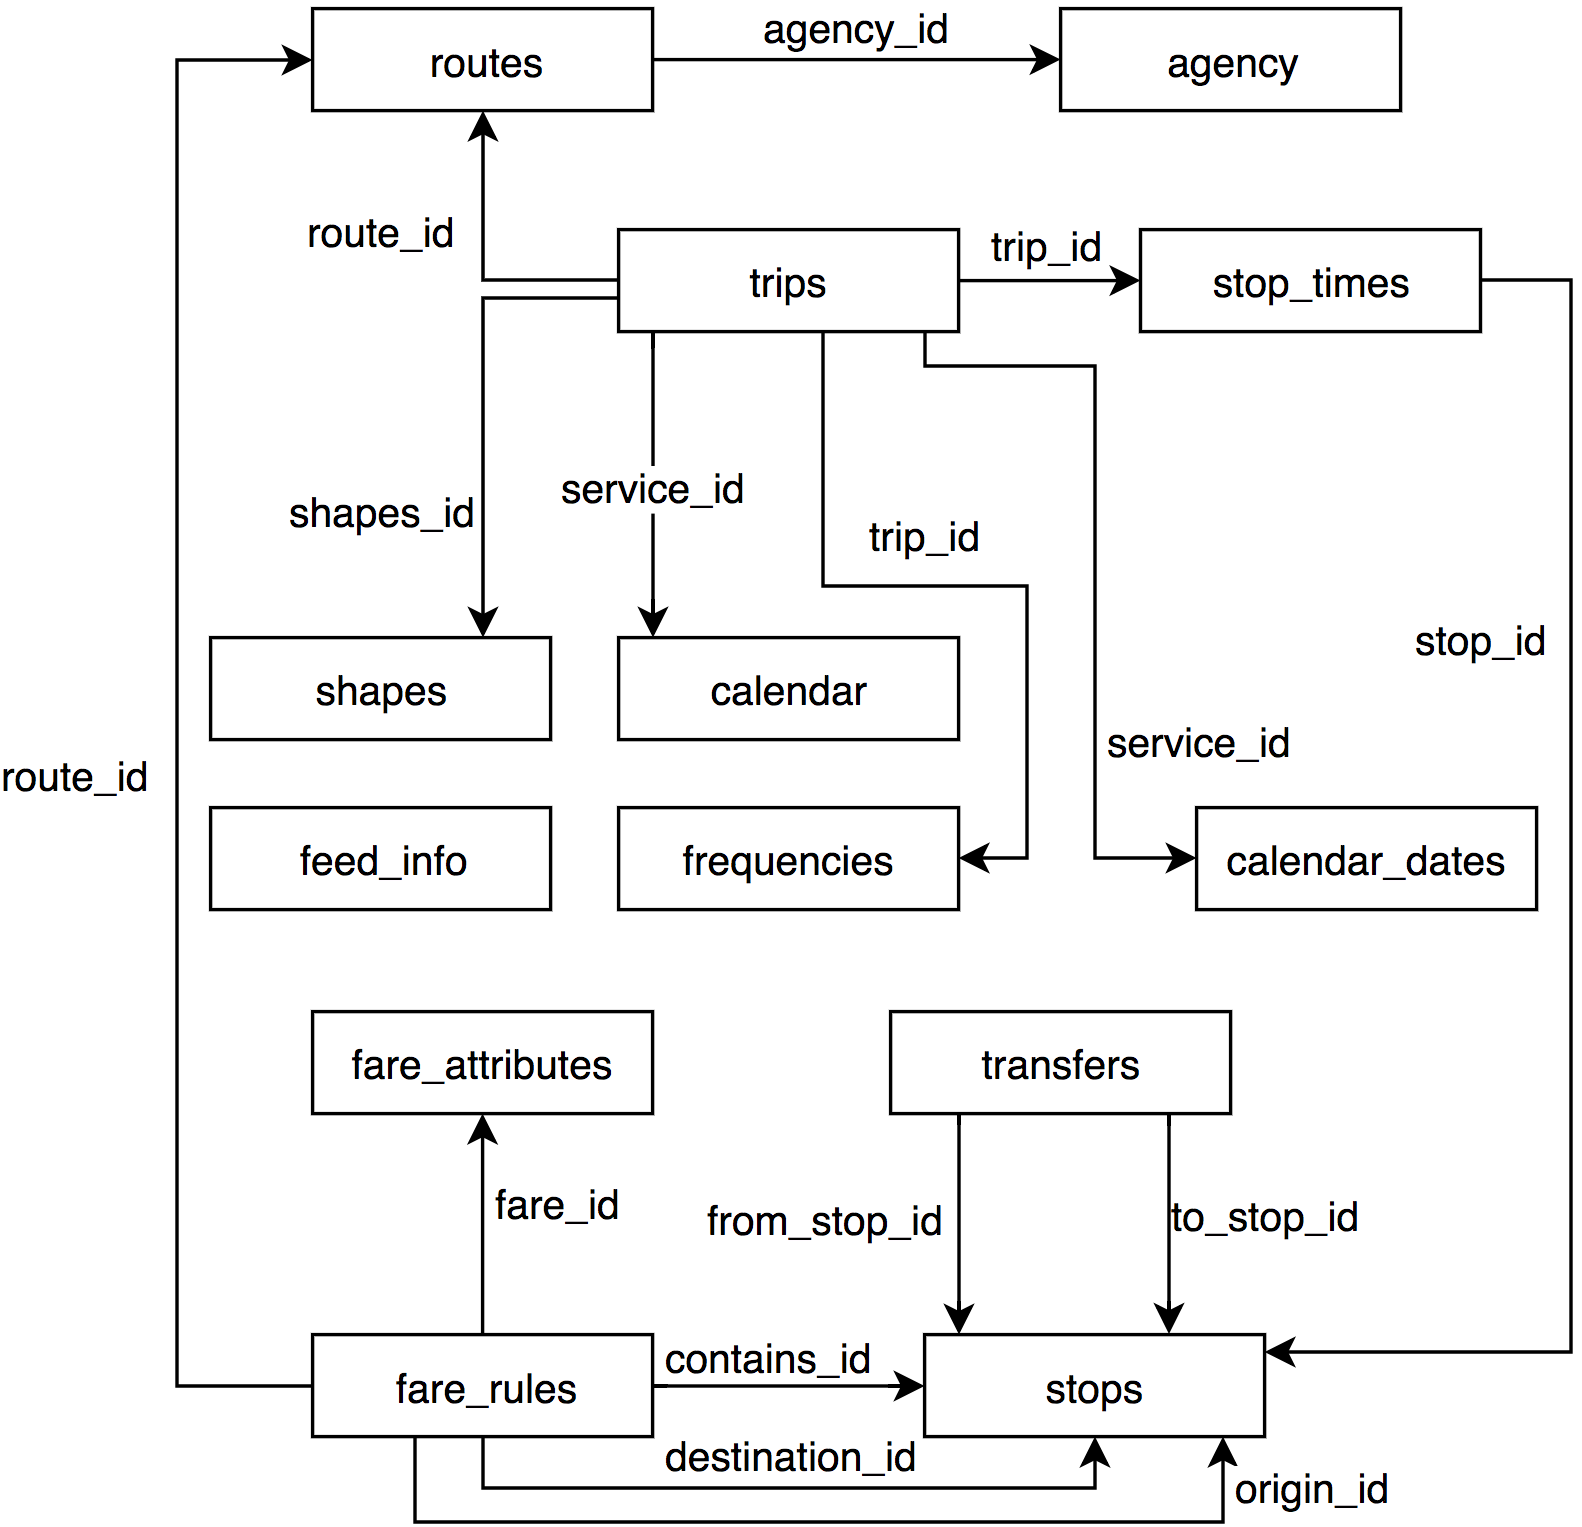
\includegraphics[width=0.47\textwidth]{images/gtfsmodel.png}
		\caption{The GTFS model and its primary relations}\label{fig:gtfs}
	\end{figure}
	
	The extension of GTFS for real-time, GTFS-RT\footnote{\url{https://developers.google.com/transit/gtfs-realtime/}} is a feed specification that allows public transport agencies to provide real time updates about their fleet. The specification supports three types of information: (i) trips updates like delays, cancellations or change routes, (ii) service alerts like stop moved, unforeseen events affecting stations, routes, etc and (iii) information of vehicle positions including location and congestion level. The data exchange format is based on Protocol Buffers\footnote{\url{https://developers.google.com/protocol-buffers/}}.
	
	It is also important to mention the works about route planning algorithms that can be developed on the top of the Linked Connections framework. The problem that these algorithms has to solve using the data is the Earliest Arrival Time (EAT). An EAT query consists of a departure stop, a departure time and a destination stop. The main goal is to find the fastest journey to the destination stop starting from the departure stop at the departure time. There are more complex route planning questions like the Minimum Expected Arrival Time (MEAT)~\cite{dibbelt2013intriguingly} or \textit{multi-criteria profile} queries~\cite{bast2010fast,delling2014round,witt2015trip}. The Connection Scan Algorithm (CSA)~\cite{dibbelt2013intriguingly} is an approach that models the timetable data as a directed acyclic graph~\cite{strasser2014connection} using a stream of connections. As we defined before, a connection is a combination of a \textit{departure stop} ($c_{depstop}$) with a \textit{departure time} ($c_{deptime}$) and an \textit{arrival stop} ($c_{arrstop}$) with an \textit{arrival time} ($c_{arrtime}$). All the connections are combined in a stream of connections, sorted by increasing departure time. Thanks to this feature, it is sufficient to only consider the connections where the $c_{deptime}$ is equals to or later than the desirable departure time. The CSA algorithm works as follows: when a new scanned connection leads to a faster route to the arrival stop, the minimum spanning tree (MST) will be updated. This is the case when $c_{arrtime}$ is earlier than the actual EAT at $c_{arrstop}$, Finally the algorithm ends when the destination stop is added to the MST and the resulting journey can be obtained by following the path in the MST backwards.
	
	In summary, after some proofs of concepts developed taking into account live and historical data in the LC framework and the current advances in the state of the work exposing the data on the Web efficiently, we think that it is the moment to improve the features of the current LC framework to create a standard mechanism for publishing reliable public transport data. The main motivations to do that are, on one hand, the necessity to improve the current access of the transport information services to the data, where at the moment that real-time is involved, the solutions are basically ad-hoc and they are not feasible if we are based on the proposal of the EU Commission for publish public transport data. On the other hand, supported by the characteristics of the transport data, where a complex data management environment emerges, the new approach that we present in this paper can serve as a source of inspiration for historical and live Linked Data management on the Web in other domains.
	
	
	\section{The Linked Connections Framework}
	In this section, we describe the Linked Connections framework for providing reliable access to live and historical data. First, we describe a summary of the Linked Connections specification including new properties about features of live data. Second, we describe the extensions we develop to deal with these types of data: the linked connections library for transforming live feeds into connections and the LC server for managing and exposing that connections on the Web efficiently.
	
	\subsection{The Linked Connections specification}
	
	The LC specification\footnote{\url{https://linkedconnections.org/specification/}} explains how to implement a data publishing sever, and explains what you can rely on when writing a route planning client. Following the Linked Data principles and the REST constraints, we make sure that from any HTTP response, hypermedia controls can be followed to discover the rest of the dataset. A "Linked Connections graph" is a paged collection of connections, describing the time transit vehicles leave and arrive. The Linked Connections vocabulary\footnote{\url{http://semweb.mmlab.be/ns/linkedconnections\#}} defines the basic properties used within the \texttt{lc:Connection} class:
	\begin{itemize}
		\item \texttt{lc:departureTime} It is a date-time, including delay, at which the vehicle will leave for the \texttt{lc:arrivalStop}.
		\item \texttt{lc:departureStop} The departure stop URI.
		\item \texttt{lc:departureDelay} Provides time in seconds when the \texttt{lc:departureTime} is not the planned departureTime.
		\item \texttt{lc:arrivalTime} It is a date-time, including delay, at which the vehicle will arrives at \texttt{lc:arrivalStop}.
		\item \texttt{lc:arrivalStop} The arrival stop URI.
		\item \texttt{lc:arrivalDelay} Provides time in second when the \texttt{lc:arrivalTime} is not the planned arrivalTime.
	\end{itemize}
	
	We also reuse the terms from the Linked GTFS vocabulary\footnote{\url{http://vocab.gtfs.org/terms}} in order to describe other properties of a \texttt{lc:Connection} class. This vocabulary it is aligned with the \textit{de-facto} standard to exchange public transport data on the Web, GTFS:
	
	\begin{itemize}
	\item \texttt{gtfs:trip} Must be set to link a \texttt{gtfs:Trip} with a \texttt{lc:Connection}, identifying whether another connection is part of the current trip of a vehicle.
	\item \texttt{gtfs:pickupType} Should be set to indicate whether people can be picked up at this stop. The possible values: \texttt{gtfs:Regular}, \texttt{gtfs:NotAvailable}, \texttt{gtfs:MustPhone} and \texttt{gtfs:MustCoordinateWithDriver}.
	\item \texttt{gtfs:dropOffType} Should be set to indicate whether people can be dropped off at this stop. The possible values are the same as the defined in the \texttt{gtfs:pickupType} property.
	\end{itemize}
	
	It is important to remark that each Linked Connections page must contain some metadata about itself. The URL after redirection, or the one indicated by the Location HTTP header, therefore must occur in the triples of the response. The current page must contain the hypermedia controls to discover under what conditions the data can be legally reused, and must contain the hypermedia controls to understand how to navigate through the paged collection(s). Different ways exist to implement the paging strategy. At least one of the strategies must be implemented for a Linked Connections client to find the next pages to be processed:
	\begin{enumerate}
	\item Each response must contain a \texttt{hydra:next} and \texttt{hydra:previous} page link.
	\item Each response should contain a \texttt{hydra:search} describing that you can search for a specific time, and that the client will be redirected to a page containing information about that timestamp. To describe this functionality the \texttt{hydra:property} \texttt{lc:departureTimeQuery} is used. An example is shown in the Figure \ref{fig:metadata}
	\end{enumerate}
	
	\begin{figure}[t]
		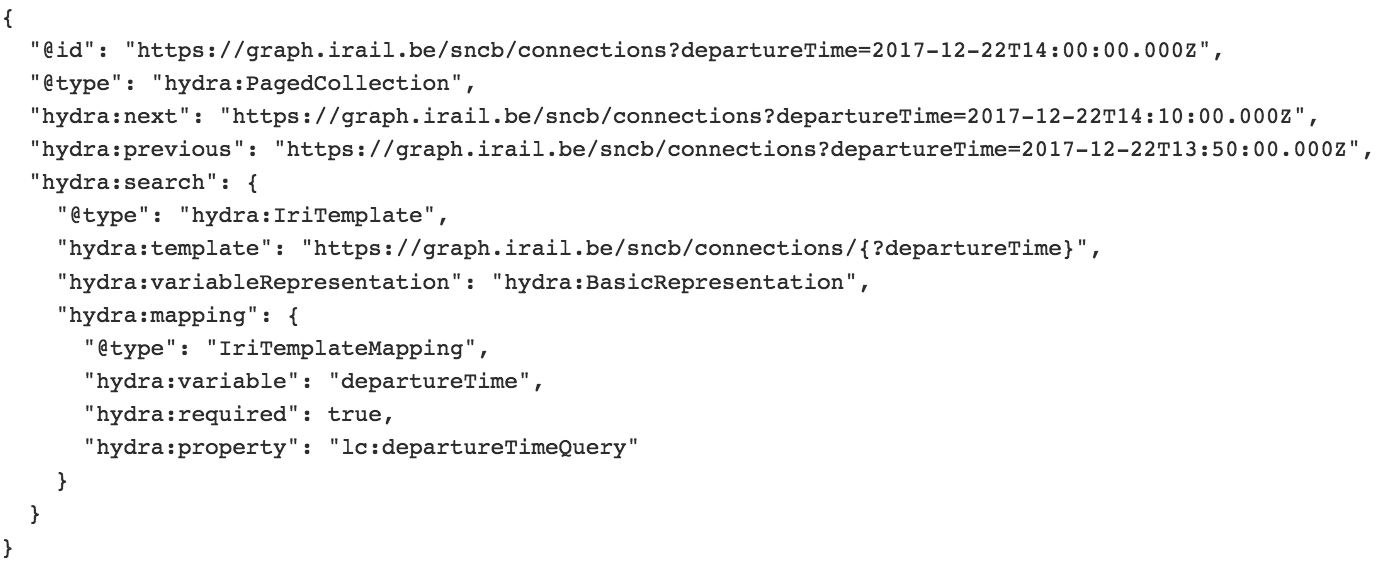
\includegraphics[width=0.5\textwidth]{images/search.png}
		\caption{Metadata LC response}\label{fig:metadata}
	\end{figure}
	
	Finally, for each document that is published by a Linked Connections server, a Cross Origin Resource Sharing\footnote{\url{http://enable-cors.org/}} HTTP header must set the property Access-Control-Allow-Origin for sharing the response with any origin. The server also should implement thorough caching strategies, as the cachability is one of the biggest advantages of the Linked Connections framework. Both conditional requests\footnote{\url{https://developer.mozilla.org/en-US/docs/Web/HTTP/Conditional_requests}} as regular caching\footnote{\url{https://developer.mozilla.org/en-US/docs/Web/HTTP/Caching}} are recommended. As every connection will need to have a unique an persistent identifier, an HTTP URI, the server must support at least one RDF1.1 format, such as JSON-LD~\cite{world2014json}, TriG~\cite{bizer2014rdf} or N-Quads~\cite{cyganiak2008n}. The connection URI should follow the Linked Data principles~\cite{bizer2009linked}.
	
	\subsection{Live data in Linked Connections}\label{real_time_lc}
	
	As we aforementioned, the transport domain should involve in their route planning algorithms the live data to provide consistent information to the passengers and improve the current informational services. The \textit{de-facto} standard for exchange transport data on the Web, GTFS, has created a version for live updates, GTFS-RT. Providing globally unique identifiers to the different entities that comprise a public transport network is fundamental to lower the adoption cost of public transport data in route-planning applications. Specifically in the case of live updates about the schedules is important to maintain stable identifiers that remain valid over time. Here we use the Linked Data principles to transform schedule updates given in the GTFS-RT format to Linked Connections and we give the option to serialize them in JSON, CSV or RDF (turtle, N-Triples or JSON-LD) format.
	
	The URI strategy to be used during the conversion process is given following the RFC 6570\footnote{\url{https://tools.ietf.org/html/rfc6570}} specification for URI templates. The parameters used to build the URIs are given following an object-like notation (object.variable) where the left side references a CSV file present in the provided GTFS data source and the right side references a specific column of such file. We use the data from a reference GTFS data source to create the URIs as with only the data present in a GTFS-RT update may not be feasible to create persistent URIs. The GFTS files that can be used to create the URIs are routes and trips files. As for the variables, any column that exists in those files can be referenced. A simple example is shown in Figure \ref{fig:connection_rt} and an standard template is also available\footnote{\url{https://github.com/linkedconnections/gtfsrt2lc/blob/master/uris_template_example.json}}. Next we describe how are the entities URIs build based on these templates :
	
	\begin{itemize}
	\item \textbf{stop}: A Linked Connection references two different stops (departure and arrival stop). The data used to build these specific URIs comes directly from the GTFS-RT update, so we do not specify any CSV file and header from the reference GTFS data source. The variable name chosen in our case is the stop\_id but it can be freely named.
	\item \textbf{route}: For the route identifier we rely on the routes.route\_short\_name and the trips.trip\_short\_name variables.
	\item \textbf{trip}: In the case of the trip we add the expected departure time on top of the route URI based on the associated connection.departureTime(YYYYMMDD) and the information about the delay.
	\item \textbf{connection}: For a connection identifier we resort to its departure stop with connection.departureStop, its departure time with connection.departureTime(YYYYMMDD), and the routes.route\_short\_name and the trips.trip\_short\_name. In this case we reference a special entity we called connection which contains the related basic data that can be extracted from a GTFS-RT update for every Linked Connection. A connection entity contains these parameters that can be used on the URIs definition: connection.departureStop, connection.arrivalStop, connection.departureTime and connection.arrivalTime. As both departureTime and arrivalTime are date objects, the expected format can be defined using brackets.
	\end{itemize}
	
	\begin{figure}[t]
		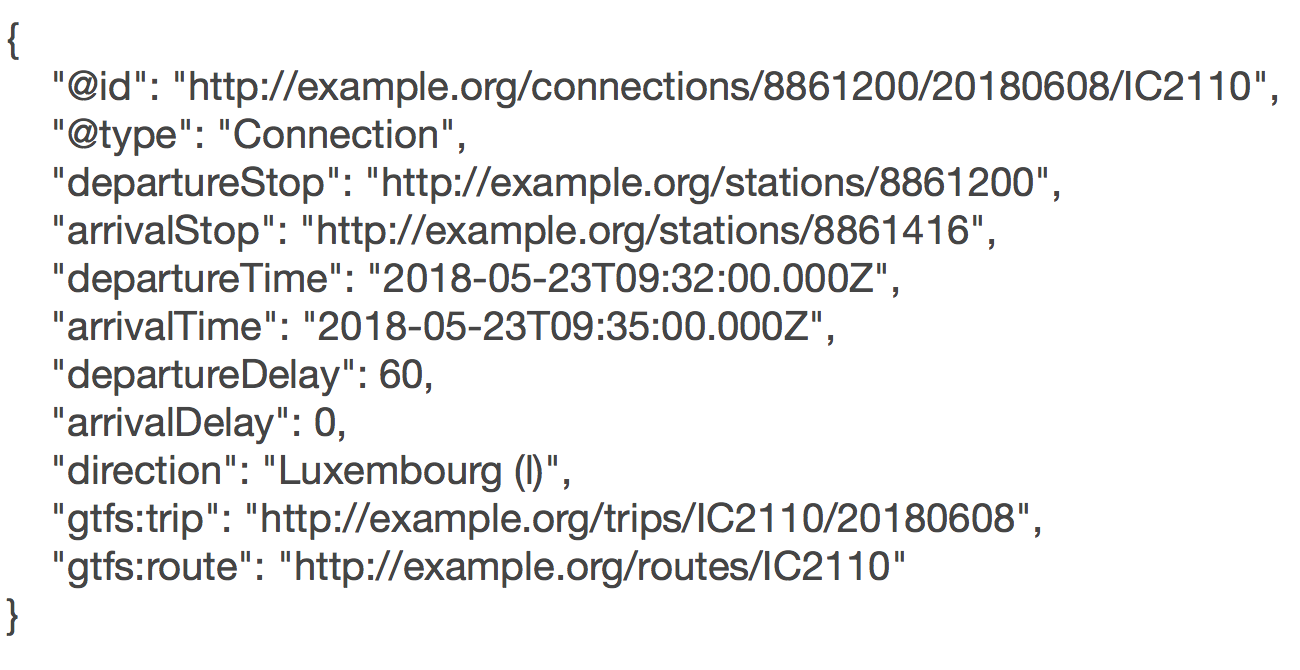
\includegraphics[width=0.47\textwidth]{images/example_connection_rt.png}
		\caption{Connection example with live updates}\label{fig:connection_rt}
	\end{figure}
	
	Finally, we developed a tool\footnote{\url{https://github.com/linkedconnections/gtfsrt2lc}} that analyses the information from an static GTFS dataset and the updates from a GTFS-RT feed, exploits the implicit relations among the CSV files and creates the live Linked Connections feed in the desirable format with the help of the URIs template, as it is shown in Figure \ref{fig:gtfsrt2lc}.
	\begin{figure}[t]
		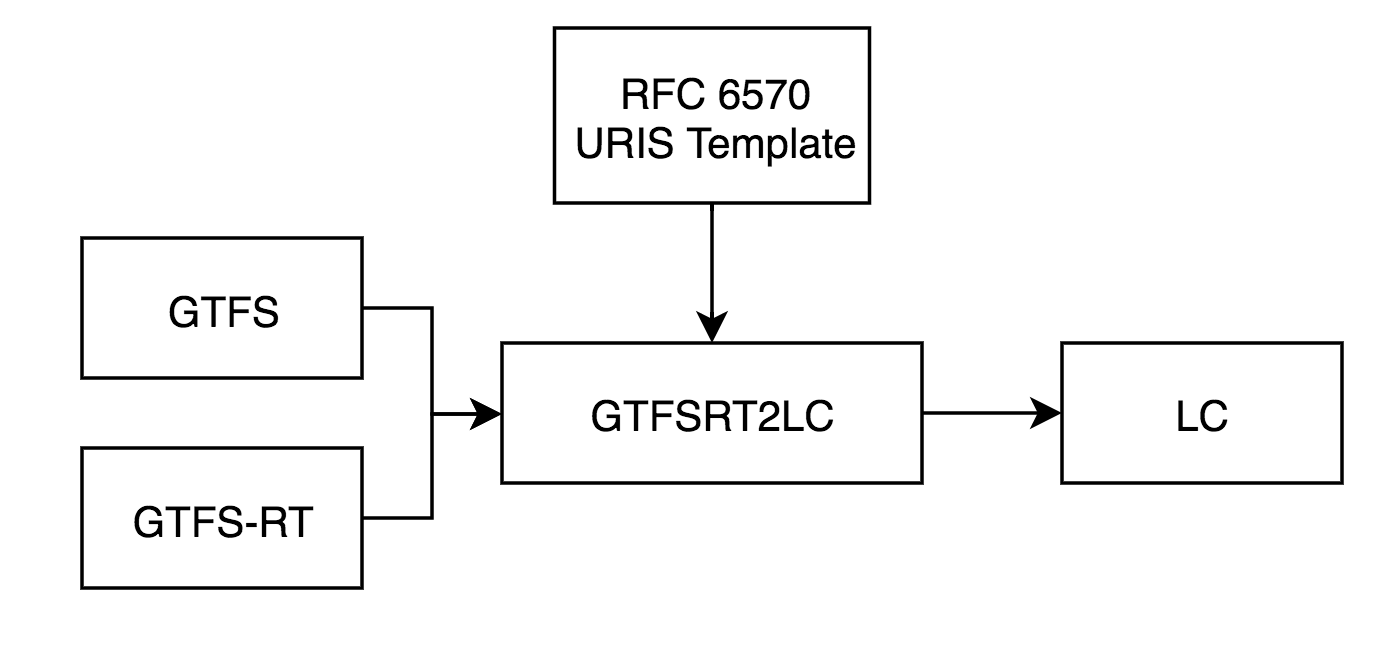
\includegraphics[width=0.47\textwidth]{images/gtfsrt2lc.png}
		\caption{The GTFSRT2LC tool}\label{fig:gtfsrt2lc}
	\end{figure}
	
	
	\subsection{Managing live and historical data with the Linked Connections server}\label{live_historical_lc}
	The third main contribution of this paper, after develop a way to create Linked Connections feeds taking into account live data, is how to provide reliable access to historical and live transport data in an cost-efficiently way. For that reason, we develop a Linked Connections server which exposes data fragments using JSON-LD serialization format. First, the server uses the GTFS2LC\footnote{\url{https://github.com/linkedconnections/gtfs2lc}} library to convert a GTFS dataset into a time sorted directed acyclic graph of connections. After that, the fragmenting process starts using the information provided in the configuration of the server about the fragment size. Once the fragmentation process is completed it starts using the GTFSRT2LC library for mapping real time updates into a Linked Connections feed as we describe in the above section. 
	
	As we aforementioned, the previous process for fragmenting LC was based on a predefined time span, which used this variable for the pagination of the data and created an heterogeneous environment in terms of the fragment size. In other words, setting a fixed time window for the creation of the fragments (e.g. 10 minutes) could lead to the creation of fragments containing a high number of connections, specially in the rush hours, and thus being big fragments in terms of size. At the same time smaller fragments could also be created at times where there are few or no vehicles departing. This is the main reason why we start to fragmenting the historical data of the LC feed homogeneously providing a specific fragment size, this has a relevant effect in terms of performance, as we demonstrate in the Section 5. As for the LC live feed we keep an unique timeline of connection updates that is stored and fragmented using a predefined time span, in contrast to static timetable updates which may contain a complete re-write or partially overlap with previous versions from a time perspective. 
	
	The server is able to manage both, the historical and the live connections. First, the server create the Linked Connections from the information provided by a GTFS dataset and fragment the historical data into several fragments. After that, if the transport system has an open live service, the sever starts to process the updates from the GTFS-RT feed and create another stream of connections based on that information. Then the server searches the correspondence between the historical and live connections based on the URIs of the trips and keeps an registry over time of the historical evolution of the connections regarding delays and/or cancellations. Finally, the server exposes the stream of historical and live connections on an API following the fragmentation approach. This process, shown in Figure \ref{fig:lc_server}, is repeated every time that the server process an update.
	
	\begin{figure}[t]
		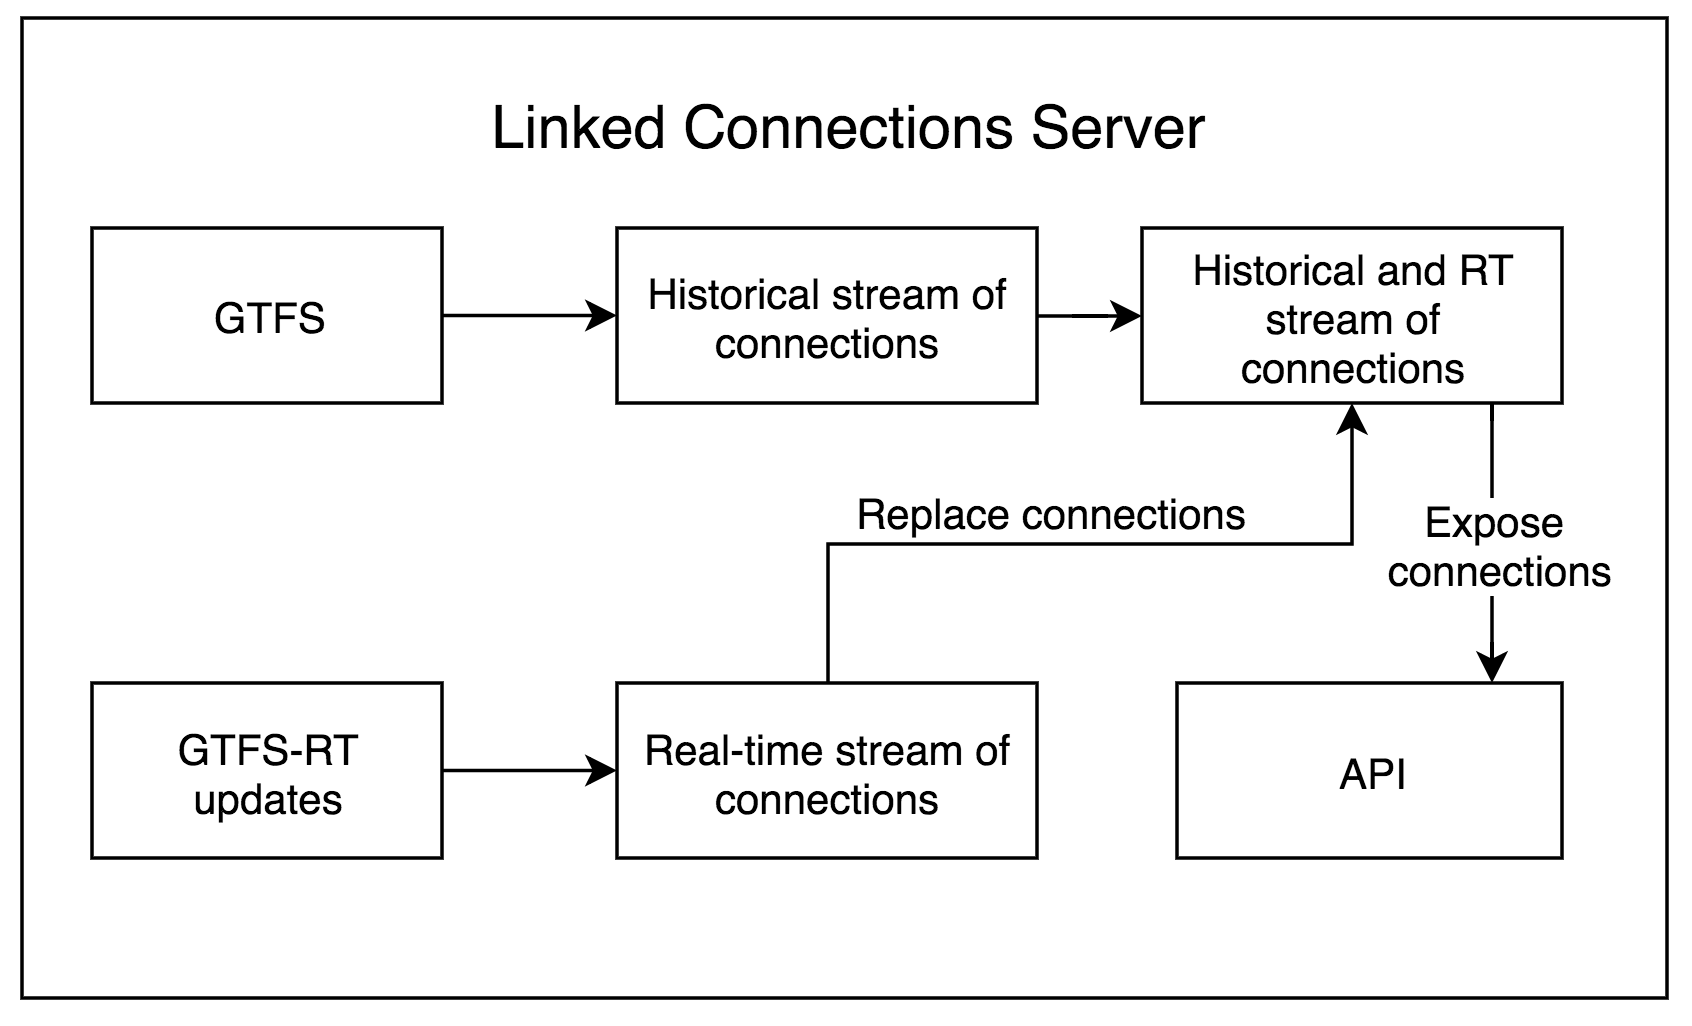
\includegraphics[width=0.47\textwidth]{images/lc_server.png}
		\caption{The Linked Connections server}\label{fig:lc_server}
	\end{figure}
	
	The server also allows querying historic data by means of the Memento Framework~\cite{van2010http} which enables time-based content negotiation over HTTP. By using the Accept-Datetime header a client can request the state of a resource at a given moment. If existing, the server will respond with a 302 Found containing the URI of the stored version of such resource. So if a request is made to obtain a Linked Connections fragment identified by a departure time, the headers of the fragment will provide the information about the Accept-Datetime. That means that is possible to know what is the state of the delays at a given date-time for a set of connections enabling different kind of analysis of the behaviour of a transport network that may contribute on the improvement of its design. This approach also guarantees the coherence of the data used to answer a give query, i.e. when a query is issued by a client, it starts to download data fragments of relevant connections to form a MST that leads to an appropriate answer, but if a new update is processed by the server while the client is still processing the query, some of the connections that the client has already processed may reappear to the client in later fragments due to updated delays, which will render invalid the MST created so far and may lead to incoherent answers. However, by using Memento and including a Accept-Datetime header in the requests made by clients, the server will guarantee that all the provided responses will belong to the same moment and will lead to valid answers. This mechanism is further described in~\cite{rojas2017providing}.    
	
	\subsection{A running example: Providing reliable access to NMBS historical and real time data}
	The NMBS is the national company of trains in Belgium. They provide their static and live data as open data in GTFS and GTFS-RT formats. We use this case to explain how our approach works.
	
	As we incorporate the GTFS2LC and GTFSRT2LC tools to the Linked Connections server, we only have to configure it to start producing the fragments of live and historical data. The basic configuration for the GTFS dataset is shown in Figure \ref{fig:nmbs_server} where the companyName must be a unique identifier of the dataset, the downloadUrl must be a public URL where the server has to download the GTFS dataset, the downloadOnLanch boolean indicates if the dataset must be downloaded and processed upon server launch, the updatePeriod is a node-cron\footnote{\url{https://www.npmjs.com/package/node-cron}} expression to check if a new version of the dataset has been published for creating a new LC feed and finally, the fragmentSize represents the size of each fragment in bytes.
	
	\begin{figure}[t]
		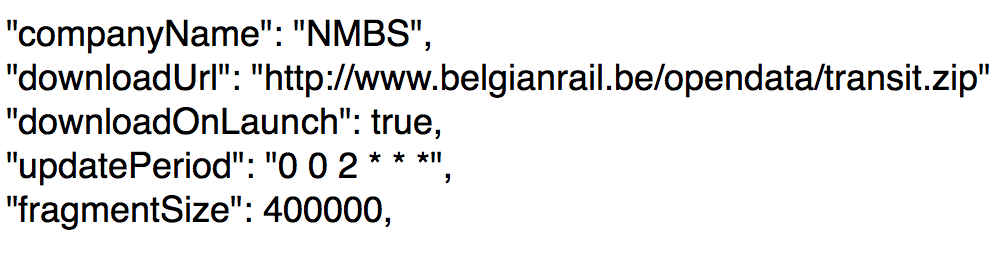
\includegraphics[width=0.47\textwidth]{images/nmbs_server.png}
		\caption{NMBS GTFS configuration}\label{fig:nmbs_server}
	\end{figure}
	
	For the GTFS-RT feed the configuration is show in the Figure \ref{fig:nmbs_rt_server} where the downloadUrl is the URL where the updates are published, the updatePeriod is a node-cron expression that indicates  how often should the server look for and process a new version of the feed, the fragmentTimeSpan defines the fragmentation of live data and it represents the time span of every fragment in seconds and finally the compressionPeriod is also a node-cron expression that defines how often will the live data be compressed using gzip in order to reduce storage consumption.
	
	\begin{figure}[t]
		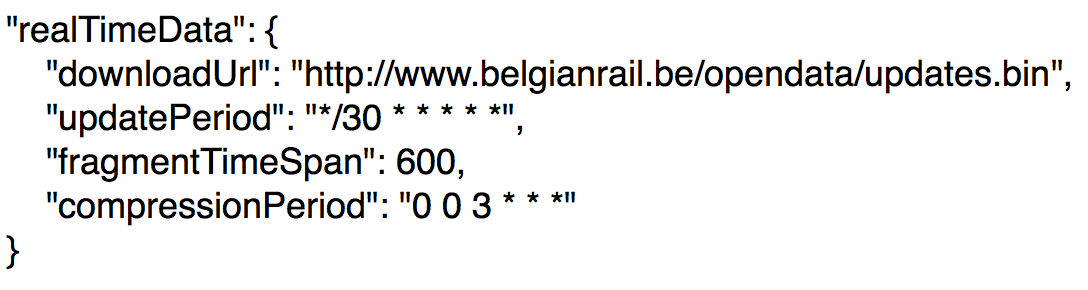
\includegraphics[width=0.47\textwidth]{images/nmbs_rt_server.png}
		\caption{NMBS GTFS-RT configuration}\label{fig:nmbs_rt_server}
	\end{figure}
	
	Finally, we have to configure the URIs using the template we describe in the Section \ref{real_time_lc} and launch the server. After the GTFS datasets have been processed, we are able to start querying the data. All the fragments have a uniform starting point, which is the expected departure time of its first \texttt{lc:connection}. So the clients can start accessing the transport data using using the departure time as a parameter like this example: \url{http://host:port/NMBS/connections?departureTime=2017-08-11T16:45:00.000Z}. In this example, we use a client implementing the CSA route planning algorithm to perform a query. The client source code is available at github\footnote{\url{https://github.com/zoeparman/connectionscan}}. The parameters of the query are as follows:
	\begin{itemize}
	\item Departure Stop: \url{http://irail.be/stations/NMBS/008811189}
	\item Arrival Stop: \url{http://irail.be/stations/NMBS/008821246}
	\item Departure Time: 2018-06-14T15:00:00.000Z
	\end{itemize}
	
	The client starts by sending a request to the server using the departure time defined in the query as a parameter for the fragments query URL. Once the server receives the request, it will determine which static fragment contains connections relevant for the query. It does this through a binary search, looking into the first connection of every fragment until it finds a fragment \(F\textsubscript{k}\) whose first connection's departure time is greater than the requested value and a fragment \(F\textsubscript{k-1}\) whose first connection's departure time is less or equal to the requested value, determining then that \(F\textsubscript{k-1}\) is the fragment to be returned in the response to client. After this, the server checks if there are live updates for the connections contained in the selected fragment and if so, it proceeds to update the departure and arrival times of the connections according to the reported delays. This process may involve the inclusion of new connections that originally belonged to previous fragments but due to the delays are now relevant for the query. In the same way some connections may have to be removed as their delays make them belong to further fragments now. Once this is done, the connections are resorted by their new departure times to ensure a correct execution of the CSA algorithm on the client side. Finally the server adds the necessary metadata (as shown on figure \ref{fig:metadata}) and gives back the response using the JSON-LD format.
	
	Once the client receives the first response, it starts looking for the first connection with a departure stop equals to the one defined in the query. When it finds one, the algorithm starts building a MST where each branch represent a different vehicle departing from the specified departure stop at a different time. The algorithm process the connections and requests new fragments for it, and if such a route exists within the transport network, eventually it will complete at least one of the branches of the MST. It will keep processing connections until the departure time of the next connections to be processed is greater than the arrival time of the fastest found route, as this means that is no longer possible to find a faster route. Finally the client will report the found routes in a JSON object as seen in figure \ref{fig:nmbs_csa}. 
	
	\begin{figure}[t]
		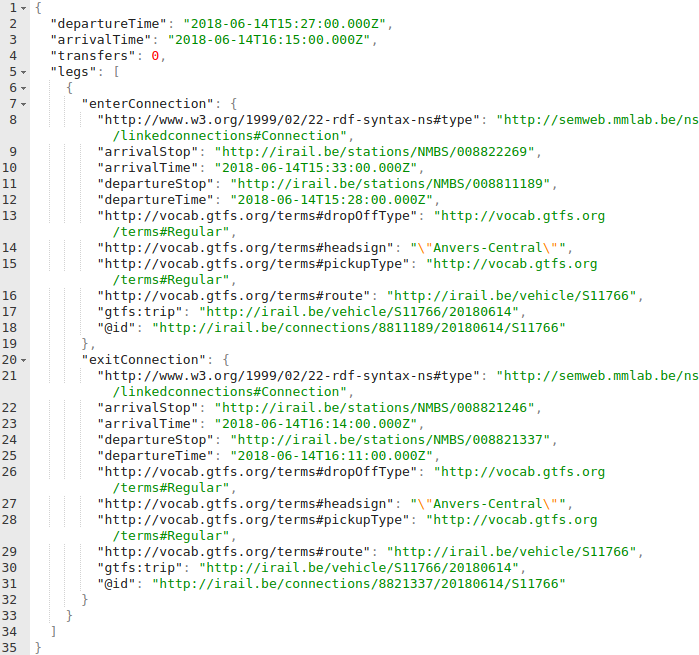
\includegraphics[width=0.47\textwidth]{images/csa_result.png}
		\caption{CSA result for a query over the NMBS Linked Connections stream}\label{fig:nmbs_csa}
	\end{figure}
	
	\section{Evaluation Design}
	
	We design a set of experiments in order to evaluate our approach. In this section we describe the main features of our developments, the data used for the experiments and the testbed we created. We implement different components in JavaScript for the Node.js platform. We chose JavaScript as it allows us to use the components both on a command-line environment as well as in the browser, which is ideal for client side applications.
	\begin{itemize}
	\item GTFSRT2LC: A tool to convert live updates and timetables as open data to Linked Connections Vocabulary.
	\item LC server: Publishes streams of connections in JSON-LD, as we explain in the Section 3.
	\item CSA algorithm: We developed the CSA algorithm on the top of the Linked Connections Framework as the client.
	\end{itemize}
	
	We also use other tools that we developed previously, as the GTFS2LC library, that it is able to convert static timetables as open data to Linked Connections Vocabulary and the Memento Protocol on the top of the Linked Connections Server~\cite{rojas2017providing}, to enable reliable access to historical data, as we describe in the Section 3.
	
	These tools are combined in different set-ups with a route planning algorithm in the client-side and are used in the following scenarios:
	\begin{itemize}
	\item Static data fragmentation by size without cache: The first experiment executes the queries taking into account only timetable static data where the size of the exposed fragments are always the same. Client caching is disabled, making this simulate the LC without cache set-up, where every request could originate from an end-user's device. We test different fragments size to test how it affects the query answering performance.
	\item Static data fragmentation by size with cache: The second experiment does the same as the first, except that it uses a client side cache, and simulates the LC with cache set-up.
	\item Historical data fragmentation by size without cache: The third experiment does the same as the first, except that it uses the Memento protocol to ensure data coherence. As the Memento protocol involves HTTP redirections to access specific resources at different points in time, this experiment is meant to measure its impact on query answering performance.
	\item Historical data fragmentation by size with cache: The fourth experiment does the same as the third, except that it uses a client side cache, and simulates the LC with cache set-up.
	\item Live and historical data fragmentation by size without cache: The fifth experiment does the same as the third, but at this tame, live data is also take into account, modifying the fragments size due to the delays. We also test different fragments sizes.
	\item Live and historical data fragmentation by size with cache: The sixth experiment does the same as the fifth except that it uses a client side cache, and simulates the LC with cache set-up.
	\item Live and historical data fragmentation by time without cache: The seventh experiment fragments the data based on time as our previous approaches with the client cache disable. We want to test if the performance of our pagination by the size is better than by time.
	\item Live and historical data fragmentation by time with cache: The eighth does the same as the seventh but it uses the client side cache.
	\end{itemize}
	
	As far as we are aware of, there are no general-purpose benchmarks in the state of the art for testing our main contributions with the Linked Connections framework. Therefore, we have created a testbed as follows: 1) we have selected and downloaded 4 different representative GTFS datasets, available as open data, that also cover several geographical locations, 2) we have created several route planning queries (departure and arrival stop with a departure time) that reflect real-life trips, with multiple levels of complexity and 3) we have evaluated these queries in the different set ups taking into account the features of each dataset. The query set created for each GTFS dataset was defined by randomly taking departure stops and arrival stops with a random departure time and using the CSA algorithm to find a route between them. This process was repeated for each transport network and spanning a 24 hours time frame of a regular week day. In the end this gave us a set of queries for each network with different levels of complexity, measured in terms of the amount of connections that need to be processed by a client to obtain a valid answer. The complexity of the queries is directly related to the complexity of the transport network itself. Meaning that the amount of connections that need to be processed in a query increase as the amount of stops and vehicles of the network also increase. Table 1 shows the characteristics (amount of stops, routes and trips) of each transport network and table 2 portrays the least and the most complex queries used during the benchmarks for each transport network.
	
	\begin{table}
	\centering
	\label{tab:datasets}
	\begin{tabular}{l|c|c|c|c}
	\hline
	\multicolumn{1}{c|}{\textbf{Dataset}} & \multicolumn{1}{c|}{\textbf{Stops}} & \multicolumn{1}{c|}{\textbf{Routes}} & \multicolumn{1}{c|}{\textbf{Trips}} & \multicolumn{1}{c}{\textbf{Connections}} \\ \hline
	TBS Barcelona & 27 & 3 & 5186 & 1957354 \\ \hline
	MLM Madrid & 81 & 4 & 2872 & 3293575 \\ \hline
	NMBS Belgium & 2615 & 479 & 12621 & 6941813 \\ \hline
	De Lijn Flanders & 36050 & 1412 & 305079 & 63006596 \\ \hline
	
	\end{tabular}
	\caption{Characteristics of the transport networks datasets used for the benchmarks.} 
	\end{table}
	
	\begin{table}
	\centering
	\label{tab:queries}
	\begin{tabular}{l|c|c}
	\hline
	\multicolumn{1}{c|}{\textbf{Query}} & \multicolumn{1}{l|}{\textbf{Dataset}} & \multicolumn{1}{l}{\textbf{\# of Connections}} \\ \hline
		\tiny depStop: http://irail.be/stations/NMBS/008841608 & \multirow{3}{*}{NMBS} & \multirow{3}{*}{3371} \\
		\tiny arrStop: http://irail.be/stations/NMBS/008841319 & & \\
		\tiny depTime: 2018-06-14T17:00:00.000Z & & \\ \hline
		\tiny depStop: http://irail.be/stations/NMBS/008886504 & \multirow{3}{*}{NMBS} & \multirow{3}{*}{13797} \\
		\tiny arrStop: http://irail.be/stations/NMBS/008841004 & & \\
		\tiny depTime: 2018-06-14T14:00:00.000Z & & \\ \hline     
		\tiny depStop: https://data.delijn.be/stops/120281 & \multirow{3}{*}{De Lijn} & \multirow{3}{*}{34696} \\
		\tiny arrStop: https://data.delijn.be/stops/126536 & & \\
		\tiny depTime: 2018-06-07T13:00:00.000Z & & \\ \hline
		\tiny depStop: https://data.delijn.be/stops/112358 & \multirow{3}{*}{De Lijn} & \multirow{3}{*}{114059} \\
		\tiny arrStop: https://data.delijn.be/stops/111446 & & \\
		\tiny depTime: 2018-06-07T13:00:00.000Z & & \\ \hline
		\tiny depStop: https://barcelona.tbs.es/stops/22 & \multirow{3}{*}{TBS} & \multirow{3}{*}{41} \\
		\tiny arrStop: https://barcelona.tbs.es/stops/21 & & \\
		\tiny depTime: 2018-06-07T20:00:00.000Z & & \\ \hline
		\tiny depStop: https://barcelona.tbs.es/stops/14 & \multirow{3}{*}{TBS} & \multirow{3}{*}{556} \\
		\tiny arrStop: https://barcelona.tbs.es/stops/10 & & \\
		\tiny depTime: 2018-06-07T05:00:00.000Z & & \\ \hline
		\tiny depStop: https://madrid.tram.es/stops/par\_10\_37 & \multirow{3}{*}{MLM} & \multirow{3}{*}{148} \\
		\tiny arrStop: https://madrid.tram.es/stops/par\_10\_32 & & \\
		\tiny depTime: 2018-06-07T21:00:00.000Z & & \\ \hline
		\tiny depStop: https://madrid.tram.es/stops/par\_10\_37 & \multirow{3}{*}{MLM} & \multirow{3}{*}{799} \\
		\tiny arrStop: https://madrid.tram.es/stops/par\_10\_26 & & \\
		\tiny depTime: 2018-06-07T16:00:00.000Z & & \\ \hline
	\end{tabular}
	\caption{Least and most complex queries of the LC testbed created for every bechmarked transport network.} 
	\end{table}
	
	The used GTFS datasets and GTFS-RT feeds are available as open data on the Web. There are two datasets that represent the Belgian Rail Transport System (NMBS) and the Flemish Transport Company (De Lijn) and other two that represent the Tram Company of Barcelona (TBS) and the Tram Company of Madrid (MLM). NMBS also provides open access to its real-time updates following the GTFS-RT format therefore, we use this data to carry out the evaluation that takes into account live updates. TBS have also developed an ad-hoc live API\footnote{\url{https://opendata.tram.cat/manual_en.pdf}} and we are currently developing a tool to transform the ad-hoc live information to the GTFS-RT format but at this moment, only historical data can be taken into account in this case. De Lijn and MLM does not provide access to their live updates which is why we only perform static and historical evaluations over this transport datasets.
	
	We ran the experiments on a laptop with an Intel Core i5-7440HQ @ 2.8GHz x 4 and 16GB of RAM. Each query is executed at least 2 times and we take the arithmetic average response time. Our experiments can be reproduced using the code at \url{https://github.com/julianrojas87/linked-connections-server} and the testbed and the data at \url{https://github.com/cef-oasis/linkedconnections-tests}.
	
	\section{Results}
	Next we present the obtained results for each of the described scenarios in the above section.
	
	\subsection{Static data with fragmentation by size}
	These results are obtained from the evaluation made over Linked Connection stream derived from GTFS datasets of each transport network. The queries executed on this evaluation do not follow the Memento protocol. We present the results for both the evaluation with and without an active client-side cache, covering the first and second experiment described above.
	
	\subsubsection{NMBS}
	For NMBS we created fragmentations of 10KB, 50KB, 300KB, 500KB, 1MB, 3MB, 7MB and 10MB. We used the same query set for both cache and no cache evaluations.
	
	\begin{figure}[h]
		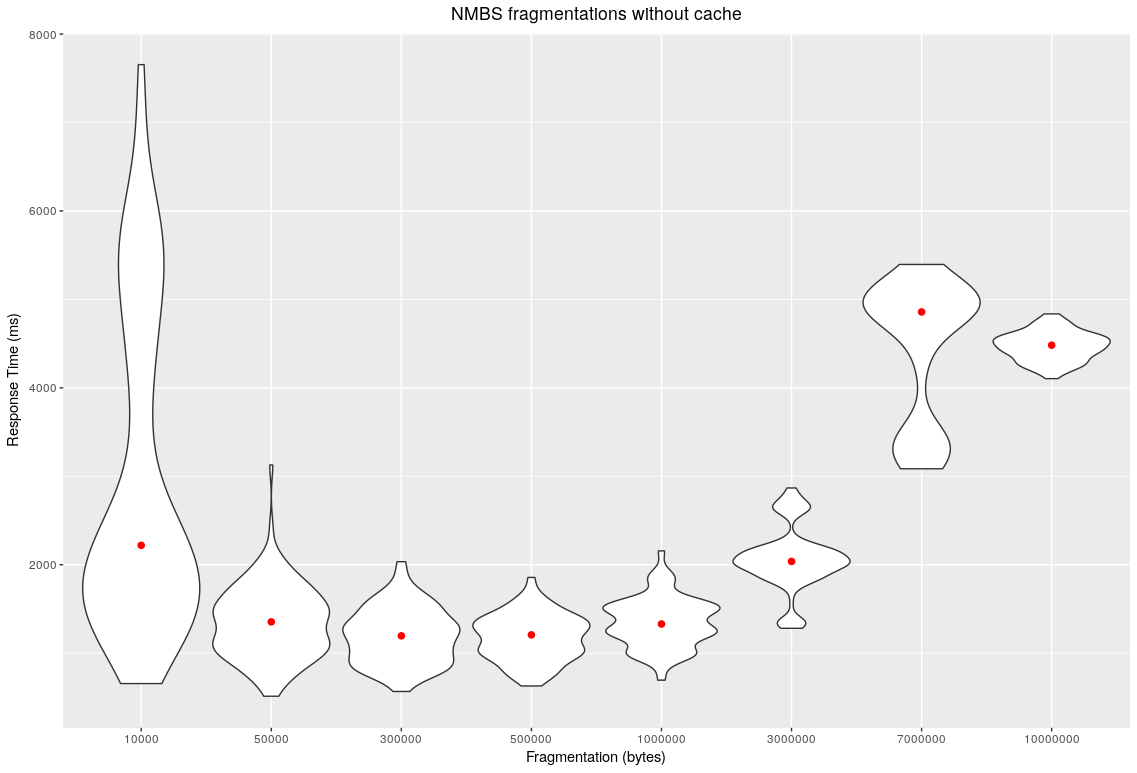
\includegraphics[width=0.47\textwidth]{nmbs/static_no_cache.png}
		\caption{NMBS static evaluation without cache}\label{fig:nmbs_static_no_cache}
	\end{figure}
	
	Figure \ref{fig:nmbs_static_no_cache} shows the response time distribution for each fragmentation in a set up without a cache. Here we have that for a fragmentation of 300KB we have the best performance with a median response time of 1196ms for the used query set. 
	
	\begin{figure}[h]
		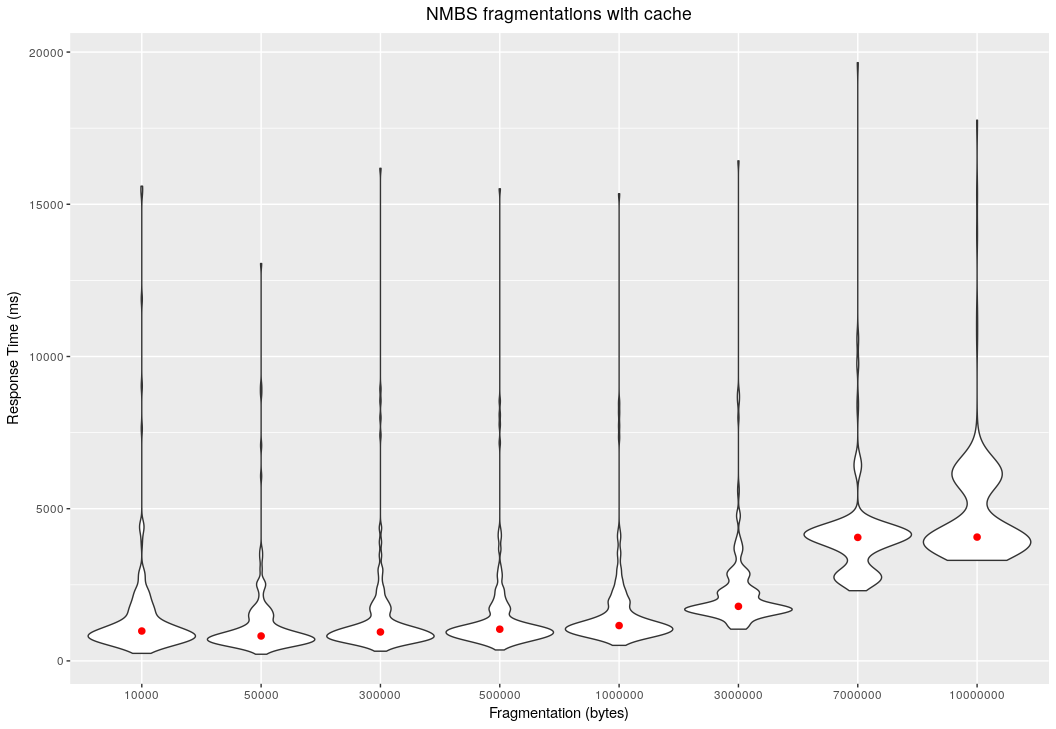
\includegraphics[width=0.47\textwidth]{nmbs/static_cache.png}
		\caption{NMBS static evaluation with cache}\label{fig:nmbs_static_cache}
	\end{figure}
	
	Figure \ref{fig:nmbs_static_cache} shows the response time distribution for each fragmentation in a set up with an active cache on the client side. In this case, the best performance was achieved with a fragmentation of 50KB and a median response time of 704ms.
	
	\subsubsection{TBS Barcelona}
	For TBS we used fragmentations going from 10KB to 3MB and we used the same query set for both cache and no cache set ups.
	
	\begin{figure}[h]
		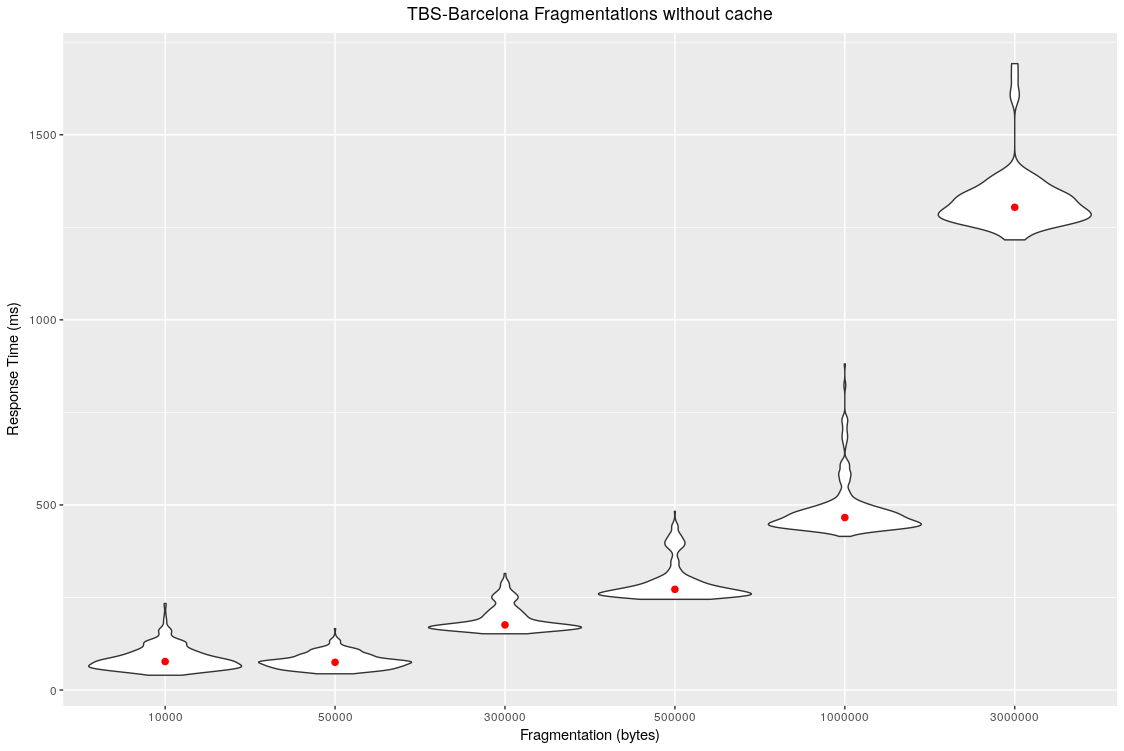
\includegraphics[width=0.47\textwidth]{tbs/no_cache.png}
		\caption{TBS static evaluation without cache}\label{fig:tbs_no_cache}
	\end{figure}
	
	Figure \ref{fig:tbs_no_cache} portrays the response time distribution for each tested fragmentation in a set up without a cache. For this case the best performance was obtained with a fragmentation of 50KB and a median response time of 75ms.
	
	\begin{figure}[h]
		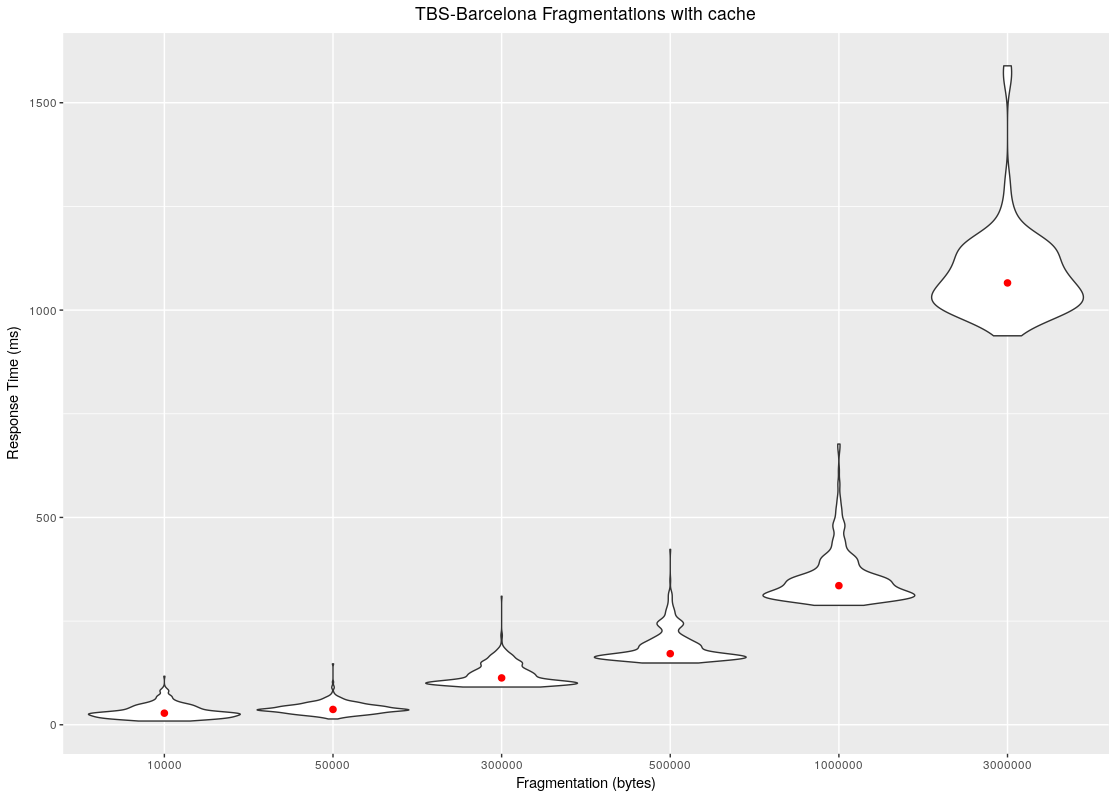
\includegraphics[width=0.47\textwidth]{tbs/cache.png}
		\caption{TBS static evaluation with cache}\label{fig:tbs_cache}
	\end{figure}
	
	Figure \ref{fig:tbs_cache} shows the response time distribution for each fragmentation in a set up with an active cache on the client side. In this case, the best performance was achieved with a fragmentation of 10KB and a median response time of 28ms.
	
	\subsubsection{MLM}
	For MLM we used fragmentations going from 10KB to 3MB and we used the same query set for both cache and no cache set ups.
	
	\begin{figure}[h]
		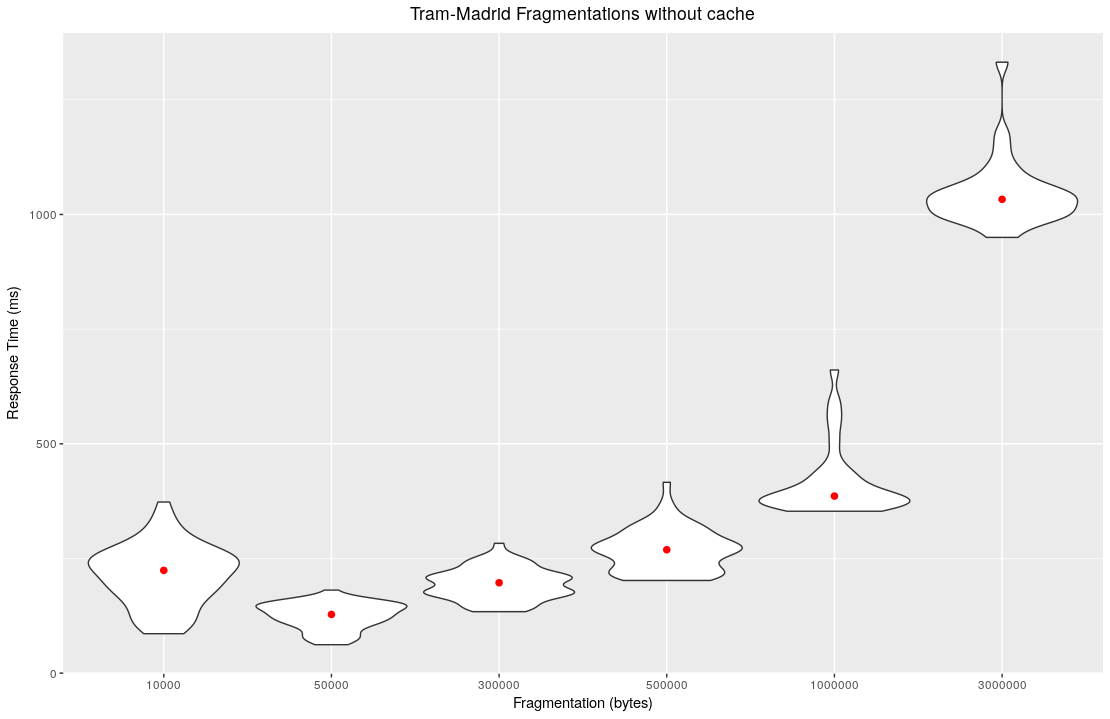
\includegraphics[width=0.47\textwidth]{mlm/static_no_cache.png}
		\caption{MLM static evaluation without cache}\label{fig:mlm_static_no_cache}
	\end{figure}
	
	Figure \ref{fig:mlm_static_no_cache} portrays the response time distribution for each tested fragmentation in a set up without a cache. For this case the best performance was obtained with a fragmentation of 50KB and a median response time of 128ms.
	
	\begin{figure}[h]
		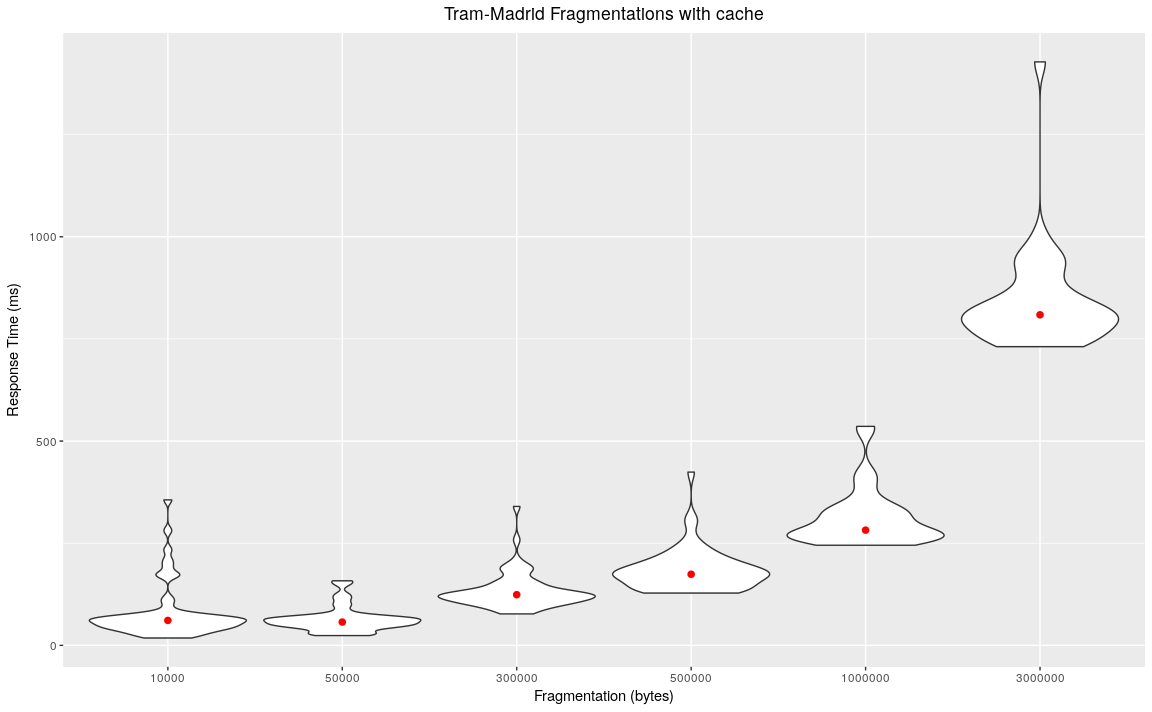
\includegraphics[width=0.47\textwidth]{mlm/static_cache.png}
		\caption{MLM static evaluation with cache}\label{fig:mlm_static_cache}
	\end{figure}
	
	Figure \ref{fig:mlm_static_cache} shows the response time distribution for each fragmentation in a set up with an active cache on the client side. In this case, the best performance was achieved with a fragmentation of 50KB and a median response time of 57ms.
	
	\subsubsection{De Lijn}
	For De Lijn the fragmentations created go from 500KB to 15MB. The query set used for the benchmarks is the same in both active and inactive cache set ups.
	
	\begin{figure}[h]
		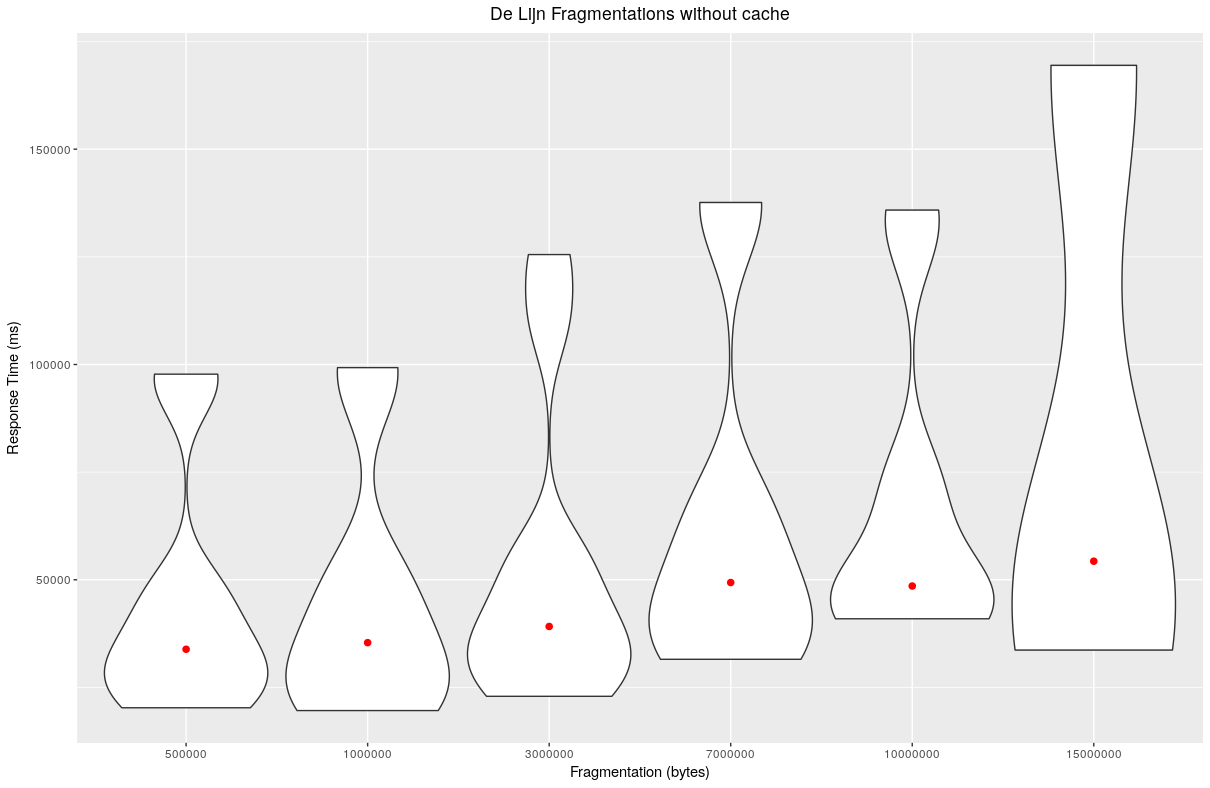
\includegraphics[width=0.47\textwidth]{delijn/no_cache.png}
		\caption{De Lijn static evaluation without cache}\label{fig:delijn_no_cache}
	\end{figure}
	
	Figure \ref{fig:delijn_no_cache} portrays the response time distribution for each tested fragmentation in a set up without a cache. For this case the best performance was obtained with a fragmentation of 500KB and a median response time of 33863ms.
	
	\begin{figure}[h]
		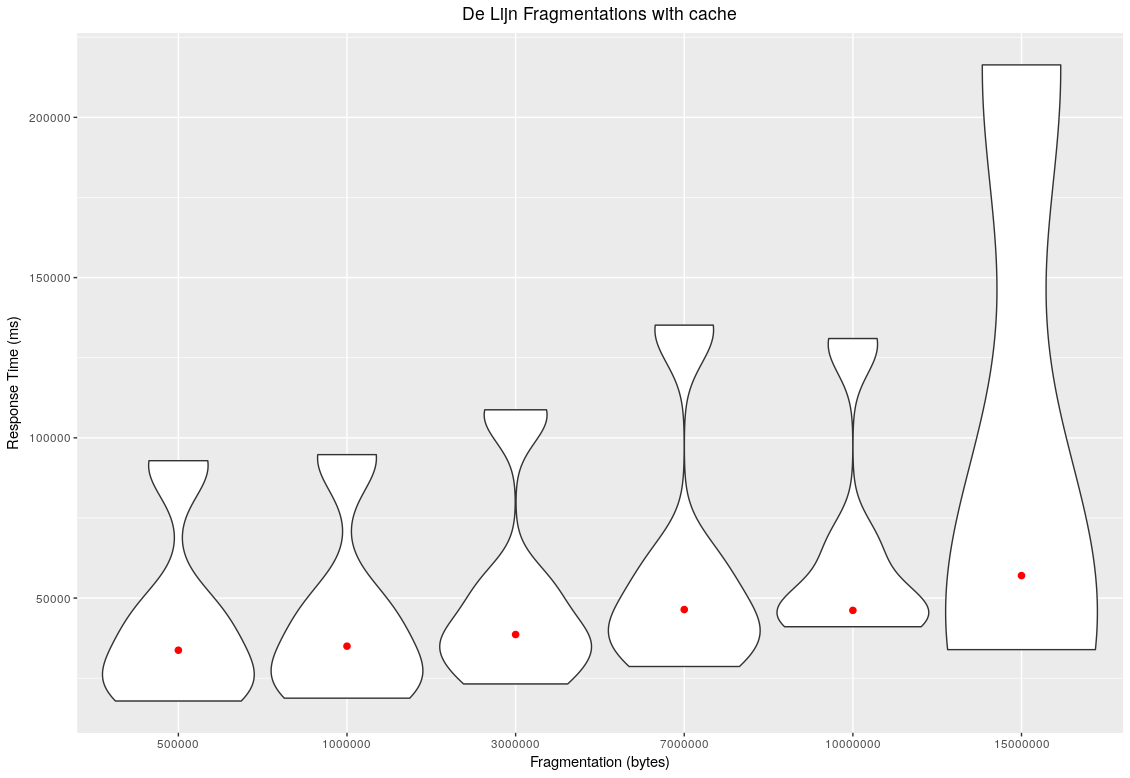
\includegraphics[width=0.47\textwidth]{delijn/cache.png}
		\caption{De Lijn static evaluation with cache}\label{fig:delijn_cache}
	\end{figure}
	
	Figure \ref{fig:delijn_cache} shows the response time distribution for each fragmentation in a set up with an active cache on the client side. In this case, the best performance was achieved with a fragmentation of 500KB and a median response time of 33729ms.
	
	\subsection{Historical data with fragmentation by size}
	The results presented here correspond to the evaluations made for historical queries on top of the NMBS and the MLM datasets. We took 3 different versions of each dataset and performed the queries defined on the query set of each transport network, but in this case the client and the server follow the Memento protocol to access historical data. By including the Accept-Datetime header on the fragment requests the client is able to calculate a route at a specific moment in time. E.g. calculate a route from Ghent to Brussels using the data as it was 3 months ago. Historical queries were tested in set ups with and without a cache. This results cover the third and fourth experiments, described in the previous section.
	
	\subsubsection{NMBS}
	In this set up we used fragmentations going from 50KB to 10MB. We performed the evaluations using an active and an inactive client-side cache.
	
	\begin{figure}[h]
		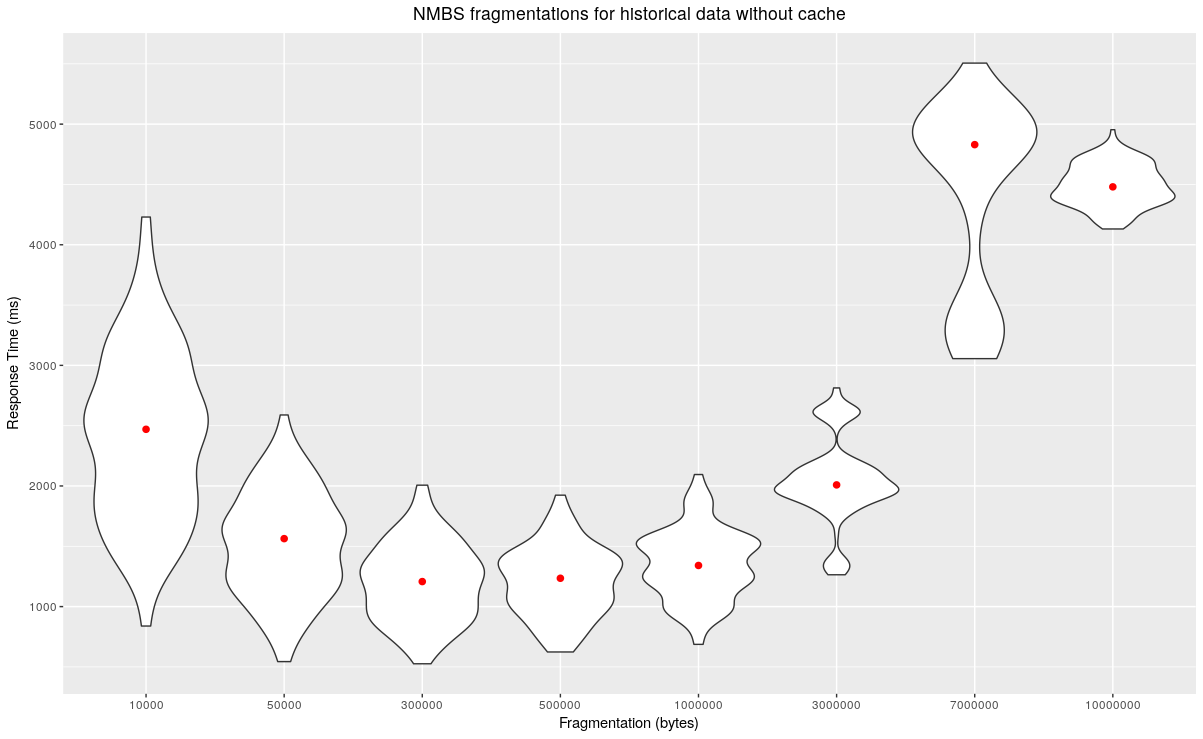
\includegraphics[width=0.47\textwidth]{nmbs/historic_no_cache.png}
		\caption{NMBS historic evaluation without cache}\label{fig:nmbs_historic_no_cache}
	\end{figure}
	
	Figure \ref{fig:nmbs_historic_no_cache} shows the response time distribution of the historical queries in a set up without a cache. The best performance is achieved with a fragmentation of 300KB and a median response time of 1207ms.
	
	\begin{figure}[h]
		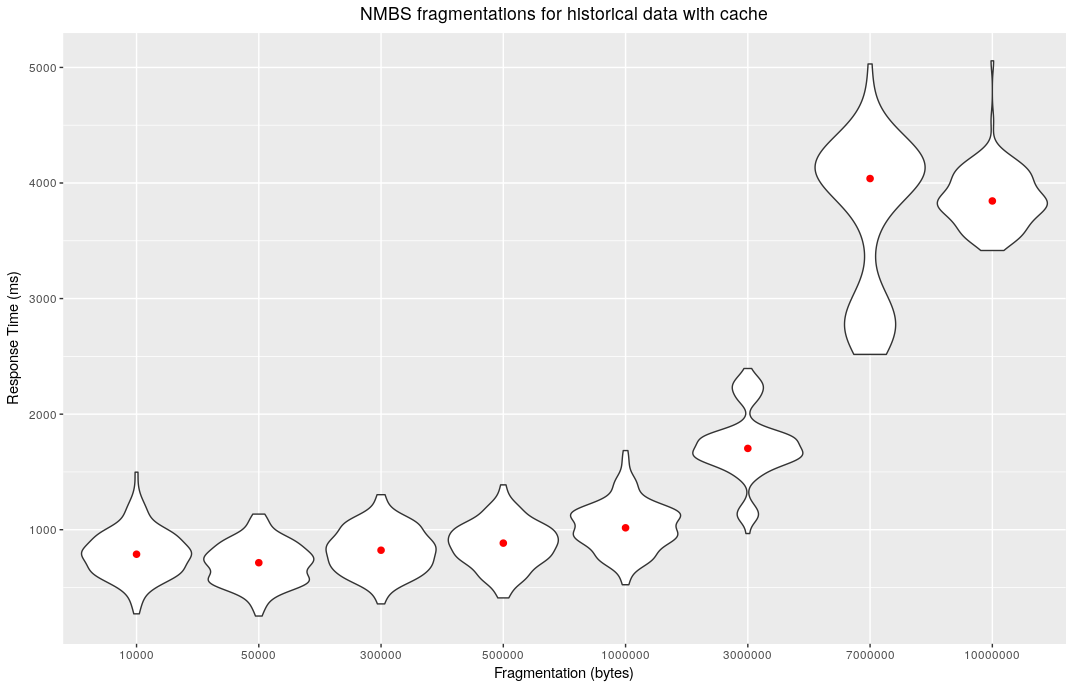
\includegraphics[width=0.47\textwidth]{nmbs/historic_cache.png}
		\caption{NMBS historic evaluation with cache}\label{fig:nmbs_historic_cache}
	\end{figure}
	
	Figure \ref{fig:nmbs_historic_cache} shows the response time distribution of the historical queries in a set up with an active cache on the client side. The best performance is achieved with a fragmentation of 50KB and a median response time of 714ms.
	
	\subsubsection{MLM}
	In this set up we used fragmentations going from 10KB to 7MB. We performed the evaluations using an active and an inactive client-side cache.
	
	\begin{figure}[h]
		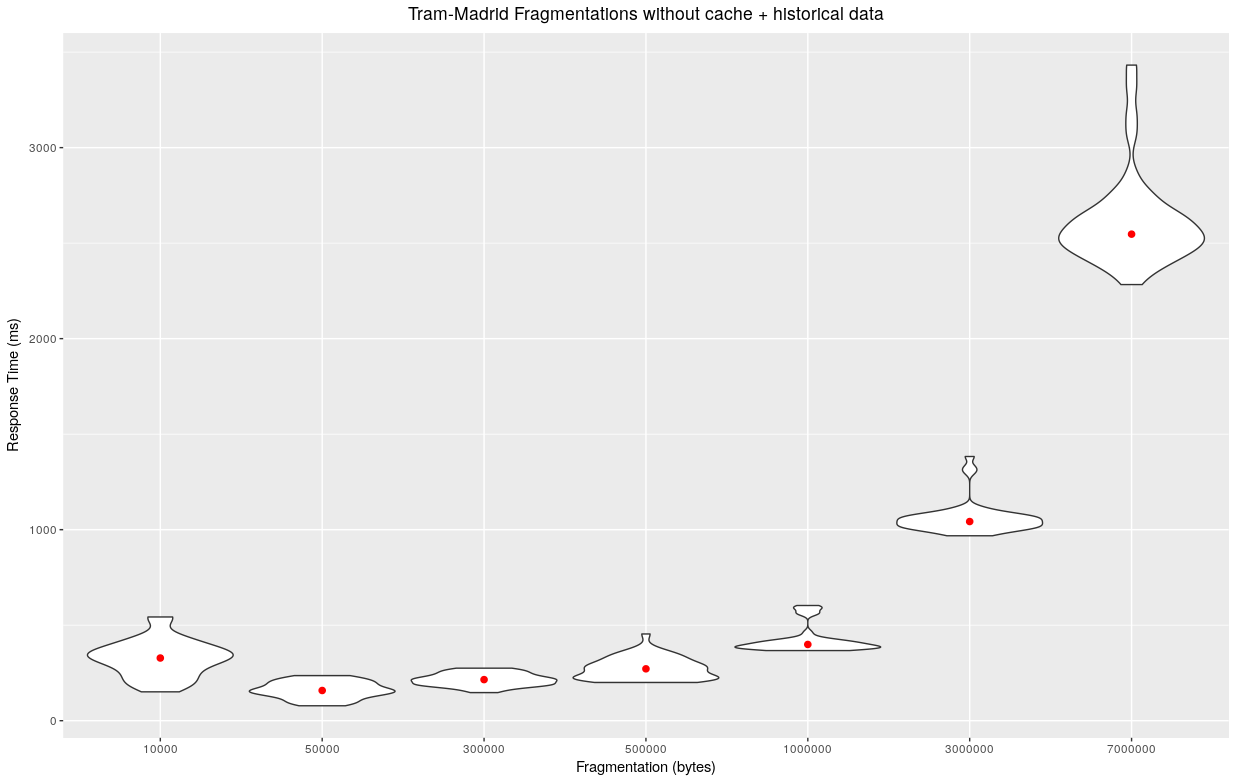
\includegraphics[width=0.47\textwidth]{mlm/historic_no_cache.png}
		\caption{MLM historic evaluation without cache}\label{fig:mlm_historic_no_cache}
	\end{figure}
	
	Figure \ref{fig:mlm_historic_no_cache} shows the response time distribution of the historical queries in a set up without a cache. The best performance is achieved with a fragmentation of 50KB and a median response time of 158ms.
	
	\begin{figure}[h]
		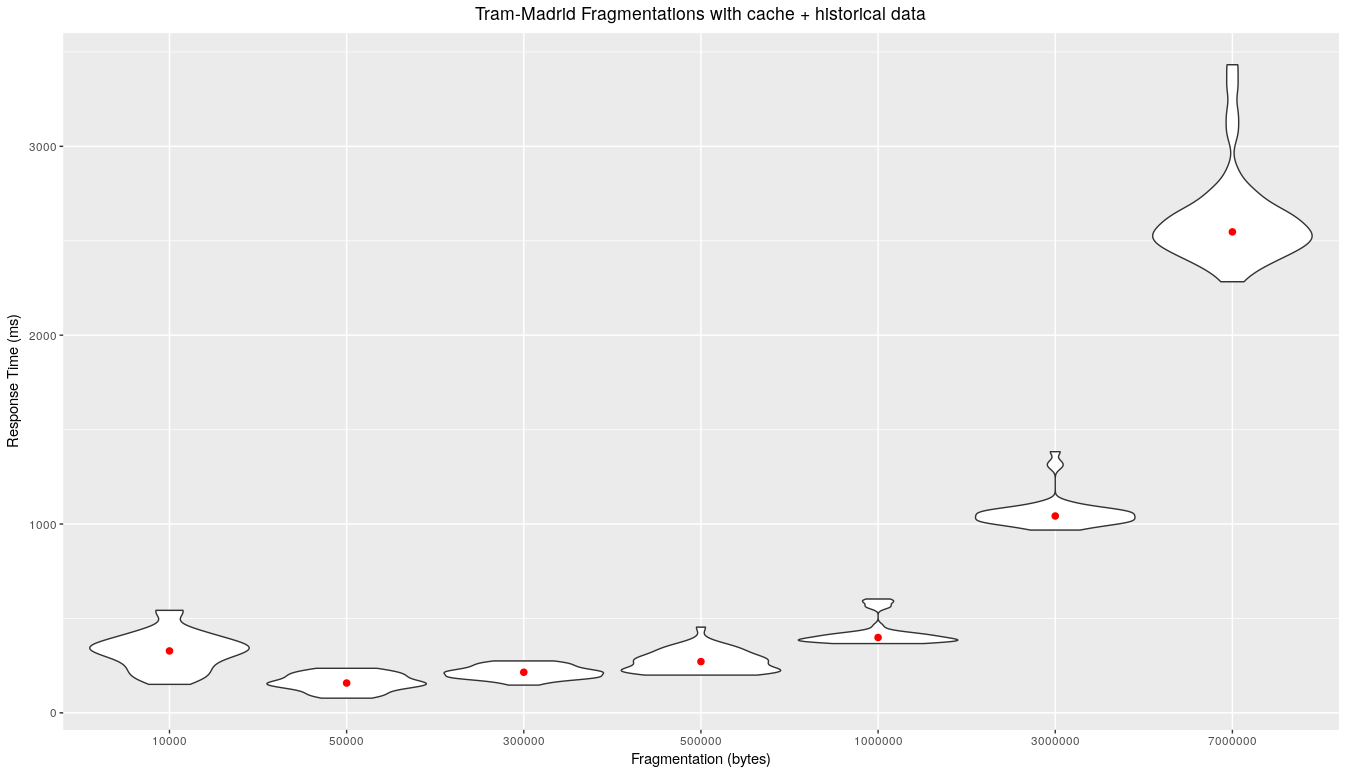
\includegraphics[width=0.47\textwidth]{mlm/historic_cache.png}
		\caption{MLM historic evaluation with cache}\label{fig:mlm_historic_cache}
	\end{figure}
	
	Figure \ref{fig:mlm_historic_cache} shows the response time distribution of the historical queries in a set up with an active cache on the client side. The best performance is achieved with a fragmentation of 50KB and a median response time of 76ms.
	
	\subsection{Live and historical data with fragmentation by size}
	The results presented here were obtained through the evaluation made over the NMBS dataset including live data. We only use the NMBS dataset as is the only one that provides a GTFS-RT feed as open data. We refer to this experiment also as historical because when we are dealing with live data, we use the Memento protocol to ensure coherence and consistency on the query answers as described in section \ref{live_historical_lc}. We test different set ups using a range of fragment sizes and measure the impact of having an active cache. This results cover the fifth ans sixth experiments, described in the previous section.
	
	\begin{figure}[h]
		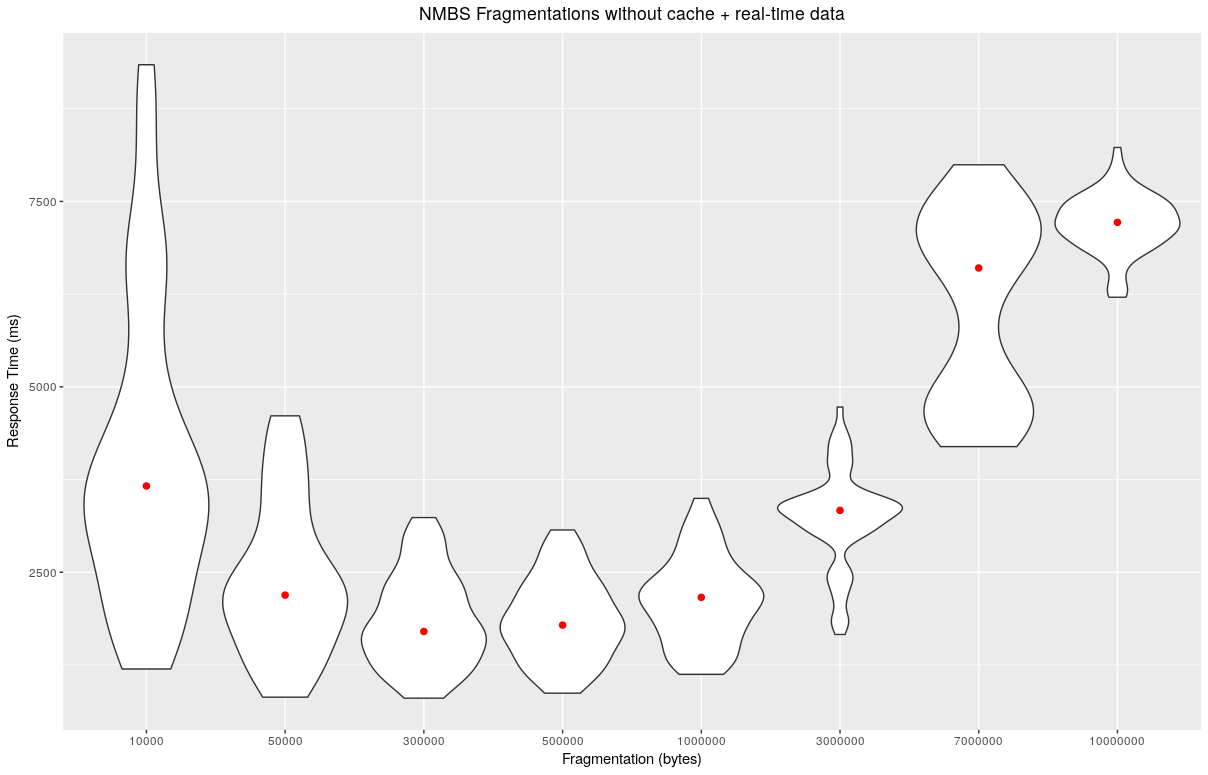
\includegraphics[width=0.47\textwidth]{nmbs/live_no_cache.png}
		\caption{NMBS live and historic evaluation without cache}\label{fig:live_no_cache}
	\end{figure}
	
	Figure \ref{fig:live_no_cache} shows the response time distribution for the live and historical queries, executed in a set up without an active cache. The best performance is obtained using a fragmentation of 300KB and a median response time of 1701ms.
	
	\begin{figure}[h]
		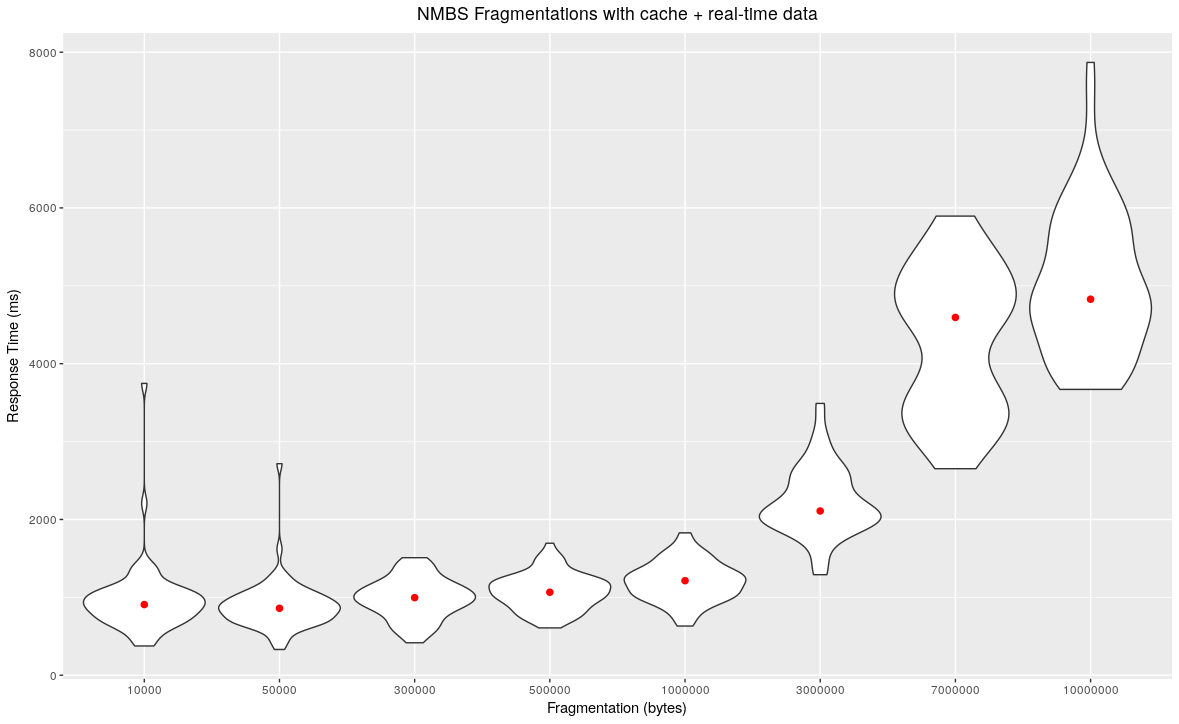
\includegraphics[width=0.47\textwidth]{nmbs/live_cache.png}
		\caption{NMBS live and historic evaluation with cache}\label{fig:live_cache}
	\end{figure}
	
	Figure \ref{fig:live_cache} shows the response time distribution for the live and historical queries, executed in a set up without an active cache. The best performance is obtained using a fragmentation of 50KB and a median response time of 859ms.
	
	\subsection{Live and historical data with fragmentation by time}
	The results presented here correspond to tests run for the NMBS transport network using their GTFS dataset and GTFS-RT feed. We defined a fragmentation for the LC stream based on a time window of 10 minutes, as we arbitrarily did in previous versions of the LC framework.
	
	\begin{figure}[h]
		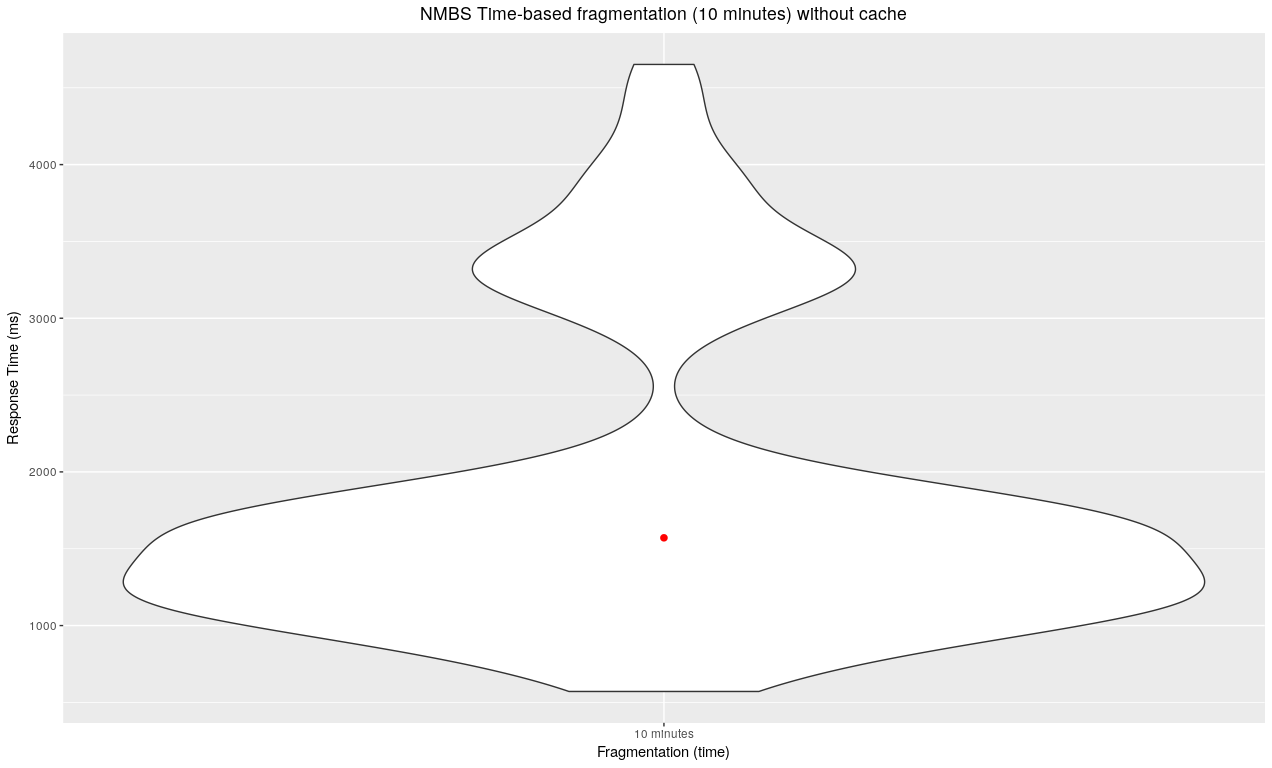
\includegraphics[width=0.47\textwidth]{nmbs/time_no_cache.png}
		\caption{NMBS live and historic evaluation based on time without cache}\label{fig:time_no_cache}
	\end{figure}
	
	Figure \ref{fig:time_no_cache} shows the response distribution for a fragmentation based on a time window of 10 minutes and we can observe a median response time of 1571ms for a set up without a cache.
	
	\begin{figure}[h]
		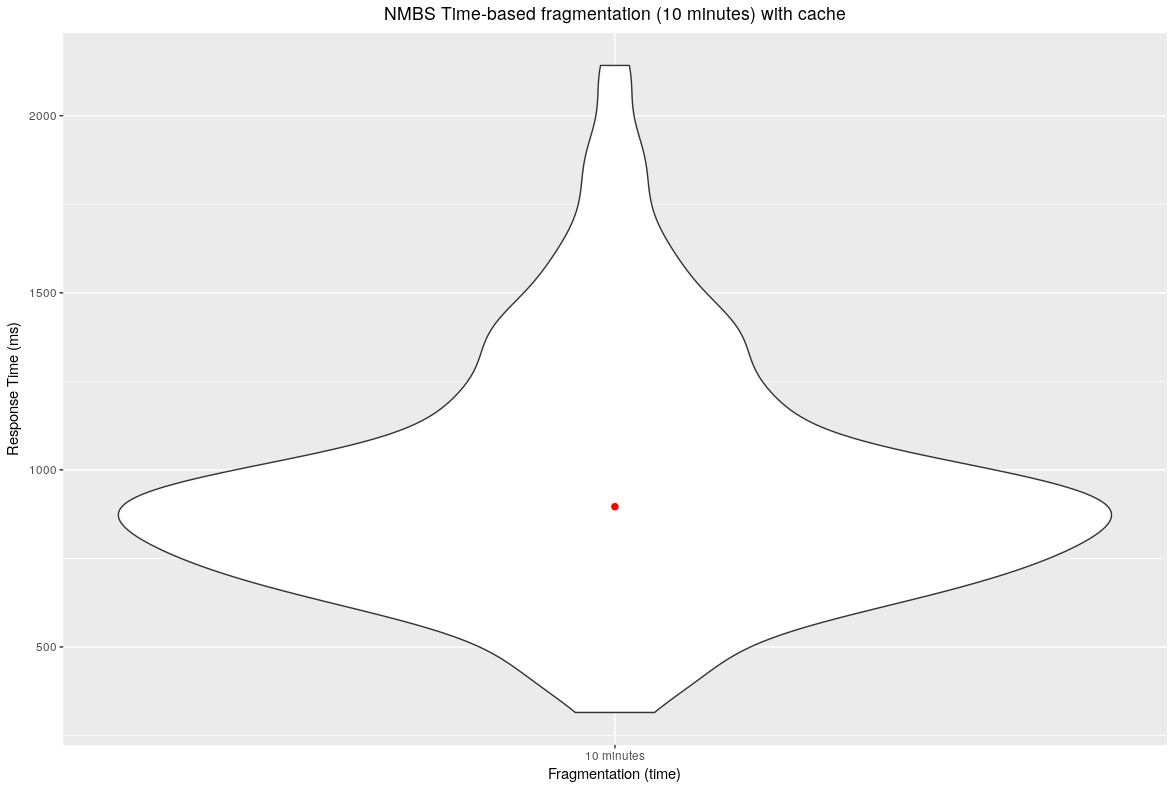
\includegraphics[width=0.47\textwidth]{nmbs/time_cache.png}
		\caption{NMBS live and historic evaluation based on time with cache}\label{fig:time_cache}
	\end{figure}
	
	Figure \ref{fig:time_cache} shows the response distribution for a fragmentation based on a time window of 10 minutes and we can observe a median response time of 896ms for a set up with an active cache.
	
	\section{Discussion}
	In the previous section we presented the results obtained for the tests we executed in 4 different scenarios. The main goal of these tests was to determine how the underlining fragmentation strategy of a LC dataset could affect the performance of route planning queries under different conditions. In previous versions of LC implementations we always used an arbitrary fragmentation strategy based on time windows of 10 minutes that lead to uneven data fragments in terms of size, which depended on the complexity of the transport network and that could affect the performance of route planning algorithms (e.g. in rush hours by having fragments too big). Therefore, we decided to move towards a fragmentation strategy based on even file sizes that allow route planners to always deal with similar fragments and thus have a more predictable behaviour. We tested different file sizes on different transport networks trying to determine an optimal fragment size on each case and also run the tests with and without an active cache to measure its impact on the performance of route planning queries. The first scenario consisted on route planning queries over LC streams derived only from GTFS datasets. We preformed these tests for all our considered transport networks (NMBS, De Lijn, TBS and MLM) in order to have a clear picture of the performance of a route planning algorithm (CSA algorithm) running on the client side and relying on an implementation of the LC specification, for transport networks of different sizes and complexities. The second scenario focused on historical queries following the Memento protocol. The capacity to query throughout different versions in time of the same dataset is an important tool for performing behavioural analysis of a transport network. We run the tests for two different transport networks (NMBS and MLM) and on each case, used three different versions of the GTFS dataset to perform historical queries. The third scenario tested the fragmentation strategies involving live data updates and measure its impact on answering route planning queries. In this case we only used the NMBS transport network as is the only company that publishes their live updates as open data and using the GTFS-RT specification. This scenario also takes into account historical queries as we use the Memento protocol when dealing with live data to maintain coherence in the query answers. Finally, the fourth scenario consisted on testing our previous fragmentation strategy based on a time window of 10 minutes and compare the performance of route planning queries with file size-based fragmentation strategies. Again, in this case we only used the NMBS transport network including live data.
	
	The results allows us to draw some generals remarks that apply for all the tested scenarios. First of all is clear in every case that using a cache has a positive impact on the performance of route planning query answering. In the case of static data we can see an improvement on the performance of 41.1\% for NMBS, 62.6\% for TBS, 55.5\% for MLM and 0.39\% for De Lijn. In the case of historical queries we have an improvement of performance of 38.6\% for NMBS and 51.8\% for MLM. In the scenario of live and historical queries we see a performance improvement of 49.5\% for NMBS. Finally, using a fragmentation based on a time window of 10 minutes, we can observe a performance improvement of 42.9\% for NMBS. Allowing the usage of caching mechanisms is one of main characteristics that the LC framework brings to the route planning ecosystem. Traditional route planning APIs based on RPC (Remote Procedure Call) architectures do not support caching as every route planning query requires a new request to the API with an unique response, in contrast to the LC framework where data fragments can be cached and reused for multiple route planning queries. Is important to highlight this result as in previous work caching proved to be a main factor for increasing server scalability and cost-efficiency for route planning applications~\cite{colpaert2017public} and now it has also proven to be a main factor for increasing the performance of route planning algorithms executed on the client side.
	
	Another general remark that can be drawn is related to the significant difference in the query response times that can be observed from one transport network to another. If we take into account the characteristics of each network (shown in table 1) we can infer that the bigger and complex a transport network is, the higher the time to answer a specific route planning query. This is an important issue from the usability perspective for route planning applications as response times that are too long could render useless all the benefits that the LC framework brings, since users won't be willing to wait that long to get an answer for a query and may resort to other route planning alternatives. In the results we can see that for a big and complex transport network as De Lijn, with 36050 stops and 1412 defined routes, the lower median response time obtained was over 33 seconds which from an usability perspective can be perceived as unacceptable. In contrast we can see that a much smaller transport network as TBS, with 27 stops and only 3 defined routes, or MLM with 81 stops and 4 defined routes achieve median response times of 28ms and 57ms respectively which, from a usability perspective is significantly fast. These results can be explained also from a geographical perspective. If we consider that the TBS network comprehends only the city of Barcelona and the MLM network is restricted only to the city of Madrid, and we compare them De Lijn which covers several cities throughout the region of Flanders in Belgium and with different transport modes, then we can justify the significant difference in query response times. For example when a query is being processed for a network as De Lijn, to go from one stop to another within the city of Ghent, the client will need to process also connections from vehicles departing in Antwerp, Bruges and all the cities that the network covers. Therefore, this results shred light over a very important requirement for the LC framework where datasets need to be as geographically restricted as possible and clients should be able to automatically select the LC streams that are relevant for a particular query, in order to maximize the query answering performance.
	
	Zooming in on the results we can also observe that for NMBS, handling historical queries and including live data increment the response time of the route planning queries. For plain static data we have a median response time of 704ms. Querying for historical data throughout different versions of a dataset raises the median response time to 714ms. And using live data for answering route planning queries raises further the median response time up to 859ms. This was the expected behaviour since using the Memento protocol for historical queries involves additional HTTP redirections for the clients which increases the processing time. In the same way, handling live data requires additional processing by the LC server to retrieve and correctly add the live updates into the data fragments before giving them back to the clients. However, we can argue that the increment measured by adding live and historical data is not significantly high from a usability perspective. For historical queries only we have an increment of 10ms and for live data we have and increment of 155ms compared to plain static data. In the same way we observe that for MLM the increment of the median response time when dealing with historical queries goes from 57ms to 76ms giving and increment of 19ms. Such increments are small enough to not be perceived by an end-user issuing a route planning query. These results represent an important achievement for the LC framework as they show that even handling historical queries and taking into account live data updates, the LC framework in conjunction with a client implementing the CSA route planning algorithm, are capable of providing an acceptable user experience for real world  route planning applications.
	
	As we previously mentioned, the main goal of these set of experiments was to determine if there is an optimal fragment size for transport network datasets that maximize the performance of answering route planning queries. Looking at the results we can observe that there is. For NMBS, that was tested in all the defined scenarios we have that 50KB fragments with an active cache always provide the best performance for route planning queries over this transport network. The same goes for the case of TBS, having 50KB fragments with an active cache as the enablers of the highest performance. In the case of MLM we have that 10KB fragments provide the best performance, however when compared to 50KB fragments, the difference is only of 9ms which can be considered not significant and can be attributed to unpredictable delays of the test environment. In the case of De Lijn we have that 500KB fragments provide the best results but then, as previously mentioned, the De Lijn dataset does not constitutes an acceptable input for the LC framework as its size and complexity cause unacceptable processing delays for a real world application and datasets with this characteristics need to be further processed in a geographical sense to be exposed as LC. Therefore we can affirm that a 50KB fragment size, with an active cache, provides the optimal performance for answering route planning queries on top of the LC framework. We can also observe that the performance decreases when moving away from this optimal point which can be explain by higher processing times when the fragment size increases and a lower probability of caching of smaller fragments. Another particular remark from these results is that when there is not an active cache available there is also an optimal point but this is higher than when there is a cache present. For the case of NMBS we see such point with fragments of 300KB which represent the balance point between the amount of requests needed for answering a query and the processing time on the client side for a given fragment. For TBS and MLM we see that the optimal point is still 50KB which seems to highlight that without a cache, there may be a relation between the optimal fragment size and the size and complexity of the transport network.
	
	Finally, we compared the performance of the NMBS dataset with historical queries and including live updates using the previous fragmentation strategy using fragments based on a time window of 10 minutes  against the current approach based on a constant fragment size. The results show that using a fragment size of 50KB and an active cache there is an improvement of 4.1\% in the performance. At first glance, this result seems to be not a significant improvement, however we need to consider that since the time-based approach does not have a constant fragment size, the performance for a given query will depend on the query itself and the complexity of the network, thus rendering the file size-based fragmentation approach more predictable and appropriate for real world route planning applications supported by the LC framework.  
	
	
	\section{Conclusions and Future work}
	In this work we present the Linked Connections framework for providing reliable access to historical and live data. First, we analyse the previous works made over the Linked Connections and their problems on efficiency when historical and live data are taken into account. Second, we extend the Linked Connections vocabulary to consider these types of data. Third, we develop a tool for creating streams of connections based on the information provided by live updates. Fourth, we adapt the LC server to efficiently manage and expose the transport data on the Web. Finally, we test our approach by analysing how the fragment size affects the performance of the CSA route planning algorithm run on the client side and compare them with our previous approach, that fragmented the data based on a time span.
	
	The conclusions that can be drawn from this work are the following:
	\begin{itemize}
	\item Using a cache mechanism significantly improves the performance of answering route planning queries using the CSA algorithm on top of an implementation of the LC framework. In previous work we were able to demonstrate the positive impact that a cache mechanism has for the scalability and cost-efficiency of a LC server compared to traditional approaches where caching is not possible. Now we have also proven how caching data fragments reduce the processing time of route planning queries as the clients keep in memory the data fragments that can be reused for answering multiple queries that are on the a similar time frame and do not have the need to request them again to the server. 
	\item The size and complexity of a transport network are directly related to the response times for answering route planning queries. We observed that as the size and complexity in terms of number of stops, routes an trips of a transport dataset increase, the response times also increase up to a point where it becomes unusable for a real world route planning application. This fact allowed us to identify a new requirement for datasets to be published as LC where the smaller and less complex the dataset, the higher the performance. This can be seen from a geographical perspective where the datasets may be also fragmented by geographical areas and also by transport modes thus lowering their complexity. However this will require the clients to have the capacity to automatically discover and consume the relevant LC sources for a specific query taking into account the involved geographical regions and transport modes.     
	\item Adding the capacity to execute historical queries by means of the Memento protocol and handling live data updates openly published using the GTFS-RT format reduce the performance of query answering as expected. However, the measured increase in the response time for viable datasets using the LC framework do not represent a significant decrease to render unusable a real world route planning application based on the LC framework.  
	\item The main conclusion drawn from this work is related to the different fragmentation strategies that may be used within the LC framework. We observed that for a set up that includes an active cache the best performance for route planning query answering is achieved by having a file size-based fragmentation of 50KB. We also observed that without a cache mechanism the optimal fragment size seems to be related to the transport network size and complexity, however as we previously mentioned, caching is a main feature of the LC framework which brings out its whole potential and differentiates it from traditional approaches.
	\item Finally, we proved that by having a constant fragment size it is possible to predict and maximize the performance of route planning query answering in the LC framework, in contrast to our previous approach where we used time-based fragmentations that created a heterogeneous environment of fragments regarding their size where the performance depends on the type of query and the complexity of the transport network.  
	\end{itemize}
	
	The LC framework stands as cost-efficient alternative to build knowledge graphs from open data in the transport sector that can be reused to build richer applications within the Web of data. By relaying on the Linked Data principles and defining a set of common semantics, the LC framework allows to publish transport datasets on the Web, optimized for route planning applications in a decentralized fashion that lower the adoption costs of the data. This establishes the foundations for creating a route planning ecosystem supported on open data that fosters innovation on the sector and aligns to the directives given by the EU regarding the discoverability and accessibility of public transport data.   
	
	For future work, we plan to develop tools/libraries able to transform other transport format standards like Datex II, Transmodel or SIRI and expose streams of connections following the LC approach on the Web. We also want to create a method able to find the optimal fragment size of a dataset based on several features like the type of the transport, the size and complexity of the full Linked Connections feed, the variability of the updates or the geographical location. Improving the discoverability of transport datasets is another line we want to take into account, we started to work on a registry by extending DCAT-AP to a Transport application profile\footnote{\url{https://github.com/cef-oasis/DCAT-AP}} to improve the discoverability of these datasets. The implementation of an usable client that can perform multimodal route planning and even take into account other types of datasets through query federation is also one of the lines of work we plan to pursue. Finally, we want to create a standard benchmarking with GTFS and GTFS-RT datasets, several representative route planning algorithms and ad-hoc relevant metrics. 
	
	\begin{acks}
	This work has been partially supported by a predoctoral grant from the I+D+i program of the Universidad Polit\'ecnica de Madrid and also by the CEF European project OASIS CEF-26696297.
	\end{acks}
	
	%\begin{figure}[t]
	%\includegraphics{}
	%\caption{Figure caption.}\label{f1}
	%\end{figure}
	
	%\begin{table*}
	%\caption{} \label{t1}
	%\begin{tabular}{lll}
	%\hline
	%&&\\
	%&&\\
	%\hline
	%\end{tabular}
	%\end{table*}
	
	%%%%%%%%%%% The bibliography starts:
	
	%%%%%%%%%%%%%%%%%%%%%%%%%%%%%%%%%%%%%%%%%%%%%%%%%%%%%%%%%%%%%
	%%                  The Bibliography                       %%
	%%                                                         %%
	%%  ios1.bst will be used to                               %%
	%%  create a .BBL file for submission.                     %%
	%%                                                         %%
	%%                                                         %%
	%%  Note that the displayed Bibliography will not          %%
	%%  necessarily be rendered by Latex exactly as specified  %%
	%%  in the online Instructions for Authors.                %%
	%%                                                         %%
	%%%%%%%%%%%%%%%%%%%%%%%%%%%%%%%%%%%%%%%%%%%%%%%%%%%%%%%%%%%%%
	
	
	\nocite{*}
	% if your bibliography is in bibtex format, use those commands:
	\bibliographystyle{ios1}           % Style BST file.
	\bibliography{bibliography}        % Bibliography file (usually '*.bib')
	
	% or include bibliography directly:
	%\begin{thebibliography}{0}
	%\bibitem{r1} F. Author, Information about cited object.
	%
	%\bibitem{r2} S. Author and T. Author, Information about cited object.
	%\end{thebibliography}
	
	\end{document}
	